%%%%%%%%%%%%%%%%%%%%%%%%%%%%%%%%%%%%%%%%%%%%%%%%%%%
%
%  New template code for TAMU Theses and Dissertations starting Fall 2012.  
%  For more info about this template or the 
%  TAMU LaTeX User's Group, see http://www.howdy.me/.
%
%  Author: Wendy Lynn Turner 
%
%%%%%%%%%%%%%%%%%%%%%%%%%%%%%%%%%%%%%%%%%%%%%%%%%%%

\documentclass[12pt]{report}
\usepackage[letterpaper]{geometry}
\geometry{verbose,tmargin=1.25in,bmargin=1.25in,lmargin=1.4in,rmargin=1.15in}
 \usepackage[doublespacing]{setspace}
 \usepackage{tocloft}
 \usepackage[rm, tiny,center, compact]{titlesec}
 \usepackage{indentfirst}
 \usepackage{etoolbox}
\usepackage{tocvsec2}
 \usepackage[titletoc]{appendix}
 \usepackage{appendix}
 \usepackage{tamuconfig}
\usepackage{rotating}

% Added to fix issues with pdf searching in some versions of LaTeX
%\usepackage[T1]{fontenc}\usepackage{lmodern}
%%%%%%%%%%%%%%%%%%%%%%%%%%%%%

\usepackage{listings}

\usepackage{color}
\definecolor{gray}{rgb}{0.4,0.4,0.4}
\definecolor{darkblue}{rgb}{0.0,0.0,0.6}
\definecolor{cyan}{rgb}{0.0,0.6,0.6}

\lstset{
  basicstyle=\ttfamily,
  columns=fullflexible,
  showstringspaces=false,
  commentstyle=\color{gray}\upshape
}

\lstdefinelanguage{XML}
{
  morestring=[b]",
  morestring=[s]{>}{<},
  morecomment=[s]{<?}{?>},
  stringstyle=\color{black},
  identifierstyle=\color{darkblue},
  keywordstyle=\color{cyan},
  morekeywords={xmlns,version,type}% list your attributes here
}

\usepackage{pbox}

\usepackage{caption}
\usepackage{subcaption}
\usepackage{breakcites}
\usepackage{url}

% Hyperref setup below.  You should be able to get away with using uncommenting just the first line.
%\usepackage[hidelinks]{hyperref}

% if \usepackage[hidelinks]{hyperref} doesn't work try this.
% \usepackage{hyperref}  % Hidelinks is an option that removes link visiability.  TAMU Thesis Offices prefers to not see the links. But often doesn't work.  
% 
% \hypersetup{
%     colorlinks=true,
%     linkcolor=black,
%     citecolor=black,
%     filecolor=black,
%     urlcolor=black,
% }
%%%%%%%  End of hyperref setup.  One of these two options should work, but my motto with hyperref is when in doubt, comment it out!
%%%%%%%%%  This hopefully fixes the problem with vertical spacing of section headings at the top of the page..  Commented out in 1.0.7
% \preto\section{%
% \ifnum\value{section}>0\addtocontents{toc}{\vskip-6pt}\fi
% }
% \preto\subsection{%
% \ifnum\value{subsection}=0\addtocontents{toc}{\vskip-6pt}\fi
% \ifnum\value{subsection}>0\addtocontents{toc}{\vskip-6pt}\fi
% } 
%%%%%%%%%%%%%%%%%%%%%%%%%%%%%%%%%%%%%%%%%%%%%%%%%%%%%%

\begin{document}

\renewcommand{\tamumanuscripttitle}{A Template-based Seismic Data Analytics Cloud Platform}
\renewcommand{\tamupapertype}{Dissertation}
\renewcommand{\tamufullname}{Yuzhong Yan}
\renewcommand{\tamudegree}{Master Degree}
\renewcommand{\tamuchairone}{Dr. Lei Huang}
% Uncomment out the next line if you have co-chairs.  You will also need to edit the titlepage.tex file.
%\newcommand{\tamuchairtwo}{Additional Chair Name}
\renewcommand{\tamumemberone}{Dr. Lei Huang}
\newcommand{\tamumembertwo}{Dr. Yonggao Yang}
\newcommand{\tamumemberthree}{Dr. Kiranmai Ballem}
\renewcommand{\tamudepthead}{Dr. Yonggao Yang}
\renewcommand{\tamugradmonth}{July}
\renewcommand{\tamugradyear}{2015}
\renewcommand{\tamudepartment}{Department of Computer Science}


%%%%%%%%%%%%%%%%%%%%%%%%%%%%%%%%%%%%%%%%%%%%%%%%%%%
%
%  New template code for TAMU Theses and Dissertations starting Fall 2012.  
%  For more info about this template or the 
%  TAMU LaTeX User's Group, see http://www.howdy.me/.
%
%  Author: Wendy Lynn Turner 
%	 Version 1.0 
%  Last updated 8/5/2012
%
%%%%%%%%%%%%%%%%%%%%%%%%%%%%%%%%%%%%%%%%%%%%%%%%%%%

%%%%%%%%%%%%%%%%%%%%%%%%%%%%%% 
%% TITLE PAGE
%% The values get updated automatically.  Please do not make changes to this file other than adding/deleting committee members where necessary.
%%%%%%%%%%%%%%%%%%%%%%%%%%%%%%

\providecommand{\tabularnewline}{\\}



\begin{titlepage}
\begin{center}
\MakeUppercase{\tamumanuscripttitle}
\vspace{4em}

A \tamupapertype

by

\MakeUppercase{\tamufullname}

\vspace{4em}

\begin{singlespace}

Submitted to the Office of Graduate and Professional Studies of \\
Texas A\&M University \\

in partial fulfillment of the requirements for the degree of \\
\end{singlespace}

\MakeUppercase{\tamudegree}
\par\end{center}
\vspace{2em}
\begin{singlespace}
\begin{tabular}{ll}
 & \tabularnewline
& \cr
% If you have Co-Chairs comment out the 'Chair of Committee' line below and uncomment the 'Co-Chairs of Committee' line.
Chair of Committee, & \tamuchairone\tabularnewline
%Co-Chairs of Committee, & \tamuchairone\tabularnewline & \tamuchairtwo\tabularnewline
Committee Members, & \tamumemberone\tabularnewline
 & \tamumembertwo\tabularnewline
 & \tamumemberthree\tabularnewline
Head of Department, & \tamudepthead\tabularnewline

\end{tabular}
\end{singlespace}
\vspace{3em}

\begin{center}
\tamugradmonth \hspace{2pt} \tamugradyear

\vspace{3em}

Major Subject: \tamudepartment \par
\vspace{3em}
Copyright \tamugradyear \hspace{.5em}\tamufullname 
\par\end{center}
\end{titlepage}
\pagebreak{}




 % This is simply a file that formats and adds your titlepage, please do not edit this unless you have a specific need. .
%%%%%%%%%%%%%%%%%%%%%%%%%%%%%%%%%%%%%%%%%%%%%%%%%%%
%
%  New template code for TAMU Theses and Dissertations starting Fall 2012.  
%  For more info about this template or the 
%  TAMU LaTeX User's Group, see http://www.howdy.me/.
%
%  Author: Wendy Lynn Turner 
%	 Version 1.0 
%  Last updated 8/5/2012
%
%%%%%%%%%%%%%%%%%%%%%%%%%%%%%%%%%%%%%%%%%%%%%%%%%%%
%%%%%%%%%%%%%%%%%%%%%%%%%%%%%%%%%%%%%%%%%%%%%%%%%%%%%%%%%%%%%%%%%%%%%
%%                           ABSTRACT 
%%%%%%%%%%%%%%%%%%%%%%%%%%%%%%%%%%%%%%%%%%%%%%%%%%%%%%%%%%%%%%%%%%%%%

\chapter*{ABSTRACT}
\addcontentsline{toc}{chapter}{ABSTRACT} % Needs to be set to part, so the TOC doesnt add 'CHAPTER ' prefix in the TOC.

\pagestyle{plain} % No headers, just page numbers
\pagenumbering{roman} % Roman numerals
\setcounter{page}{2}

\indent Lorem ipsum dolor sit amet, consectetur adipiscing elit. Integer lectus quam, condimentum quis bibendum eu, sollicitudin eget lacus. Praesent non sodales odio. Class aptent taciti sociosqu ad litora torquent per conubia nostra, per inceptos himenaeos. Nulla ac luctus sapien. Morbi cursus sapien eget lorem fermentum hendrerit. Nam ac erat dui, in cursus velit. Vivamus hendrerit porttitor nisi, ut porttitor lorem volutpat eget. In ligula ligula, euismod ut condimentum sit amet, pulvinar sit amet diam. Pellentesque interdum, ipsum ullamcorper consequat dignissim, sem arcu egestas mauris, vitae interdum sem tortor ut ante. Nunc blandit laoreet nisi, non rutrum lorem hendrerit quis. Cras nunc diam, convallis et feugiat at, auctor id libero. Nunc facilisis massa eu eros imperdiet vestibulum. Vestibulum ante ipsum primis in faucibus orci luctus et ultrices posuere cubilia Curae; Donec non velit vitae tortor blandit semper.

Etiam vitae dolor nulla. Ut eros odio, rhoncus eget placerat vitae, elementum ac ante. Proin vitae odio eu nisl pharetra mattis. Pellentesque habitant morbi tristique senectus et netus et malesuada fames ac turpis egestas. Phasellus fermentum lacus consectetur neque consequat ullamcorper. Cras blandit urna non dui consequat molestie. Curabitur viverra nibh at nisi semper faucibus. Nam egestas mauris a enim dignissim nec consectetur tortor rutrum. Mauris at nisi in est luctus congue ut mattis est. Ut pretium, mi quis elementum cursus, ante eros suscipit ligula, ut porttitor elit leo sed turpis. Nam sed dui ligula.

 

\pagebreak{}

%%%%%%%%%%%%%%%%%%%%%%%%%%%%%%%%%%%%%%%%%%%%%%%%%%%%
%
%  New template code for TAMU Theses and Dissertations starting Fall 2012.  
%  For more info about this template or the 
%  TAMU LaTeX User's Group, see http://www.howdy.me/.
%
%  Author: Wendy Lynn Turner 
%	 Version 1.0 
%  Last updated 8/5/2012
%
%%%%%%%%%%%%%%%%%%%%%%%%%%%%%%%%%%%%%%%%%%%%%%%%%%%

%%%%%%%%%%%%%%%%%%%%%%%%%%%%%%%%%%%%%%%%%%%%%%%%%%%%%%%%%%%%%%%%%%%%%%
%%                           DEDICATION
%%%%%%%%%%%%%%%%%%%%%%%%%%%%%%%%%%%%%%%%%%%%%%%%%%%%%%%%%%%%%%%%%%%%%
\chapter*{DEDICATION}
\addcontentsline{toc}{chapter}{DEDICATION}  % Needs to be set to part, so the TOC doesnt add 'CHAPTER ' prefix in the TOC.



\indent This is an optional page.  Lorem ipsum dolor sit amet, consectetur adipiscing elit. Integer lectus quam, condimentum quis bibendum eu, sollicitudin eget lacus. Praesent non sodales odio. Class aptent taciti sociosqu ad litora torquent per conubia nostra, per inceptos himenaeos. Nulla ac luctus sapien. Morbi cursus sapien eget lorem fermentum hendrerit. Nam ac erat dui, in cursus velit. Vivamus hendrerit porttitor nisi, ut porttitor lorem volutpat eget. In ligula ligula, euismod ut condimentum sit amet, pulvinar sit amet diam. Pellentesque interdum, ipsum ullamcorper consequat dignissim, sem arcu egestas mauris, vitae interdum sem tortor ut ante. Nunc blandit laoreet nisi, non rutrum lorem hendrerit quis. Cras nunc diam, convallis et feugiat at, auctor id libero. Nunc facilisis massa eu eros imperdiet vestibulum. Vestibulum ante ipsum primis in faucibus orci luctus et ultrices posuere cubilia Curae; Donec non velit vitae tortor blandit semper.

Etiam vitae dolor nulla. Ut eros odio, rhoncus eget placerat vitae, elementum ac ante. Proin vitae odio eu nisl pharetra mattis. Pellentesque habitant morbi tristique senectus et netus et malesuada fames ac turpis egestas. Phasellus fermentum lacus consectetur neque consequat ullamcorper. Cras blandit urna non dui consequat molestie. Curabitur viverra nibh at nisi semper faucibus. Nam egestas mauris a enim dignissim nec consectetur tortor rutrum. Mauris at nisi in est luctus congue ut mattis est. Ut pretium, mi quis elementum cursus, ante eros suscipit ligula, ut porttitor elit leo sed turpis. Nam sed dui ligula.


\pagebreak{}

%%%%%%%%%%%%%%%%%%%%%%%%%%%%%%%%%%%%%%%%%%%%%%%%%%%
%
%  New template code for TAMU Theses and Dissertations starting Fall 2012.  
%  For more info about this template or the 
%  TAMU LaTeX User's Group, see http://www.howdy.me/.
%
%  Author: Wendy Lynn Turner 
%	 Version 1.0 
%  Last updated 8/5/2012
%
%%%%%%%%%%%%%%%%%%%%%%%%%%%%%%%%%%%%%%%%%%%%%%%%%%%


%%%%%%%%%%%%%%%%%%%%%%%%%%%%%%%%%%%%%%%%%%%%%%%%%%%%%%%%%%%%%%%%%%%%%%
%%                           ACKNOWLEDGEMENTS
%%%%%%%%%%%%%%%%%%%%%%%%%%%%%%%%%%%%%%%%%%%%%%%%%%%%%%%%%%%%%%%%%%%%%
\chapter*{ACKNOWLEDGEMENTS}
\addcontentsline{toc}{chapter}{ACKNOWLEDGEMENTS}  % Needs to be set to part, so the TOC doesnt add 'CHAPTER ' prefix in the TOC.

Please find below the list of the persons you should acknowledged:

 

Supervisors (main and second)
Academic staff in your department
Technical staff
Academic staff
Colleagues
Institutions and organization
Companies
Family and friends

\pagebreak{}

%%%%%%%%%%%%%%%%%%%%%%%%%%%%%%%%%%%%%%%%%%%%%%%%%%%%
%
%  New template code for TAMU Theses and Dissertations starting Fall 2012.  
%  For more info about this template or the 
%  TAMU LaTeX User's Group, see http://www.howdy.me/.
%
%  Author: Wendy Lynn Turner 
%	 Version 1.0 
%  Last updated 8/5/2012
%
%%%%%%%%%%%%%%%%%%%%%%%%%%%%%%%%%%%%%%%%%%%%%%%%%%%

%%%%%%%%%%%%%%%%%%%%%%%%%%%%%%%%%%%%%%%%%%%%%%%%%%%%%%%%%%%%%%%%%%%%%%
%%                           NOMENCLATURE
%%%%%%%%%%%%%%%%%%%%%%%%%%%%%%%%%%%%%%%%%%%%%%%%%%%%%%%%%%%%%%%%%%%%%

\chapter*{NOMENCLATURE}
\addcontentsline{toc}{chapter}{NOMENCLATURE}  % Needs to be set to part, so the TOC doesnt add 'CHAPTER ' prefix in the TOC.

\begin{tabular}{ll}
B/CS  & Bryan/College Station\tabularnewline
HSUS & Humane Society of the United States\tabularnewline
P & Pressure\tabularnewline
T  & Time\tabularnewline
TVA & Tennessee Valley Authority\tabularnewline
TxDOT \hfill{}\hfill{}\hfill{}\hfill{}\hfill{}\hfill{}\hfill{}\hfill{} & \multicolumn{1}{l}{Texas Department of Transportation}\tabularnewline
\end{tabular}

\vspace{2em}

This page is optional.

\pagebreak{}

%%%%%%%%%%%%%%%%%%%%%%%%%%%%%%%%%%%%%%%%%%%%%%%%%%%
%
%  New template code for TAMU Theses and Dissertations starting Fall 2012.  
%  For more info about this template or the 
%  TAMU LaTeX User's Group, see http://www.howdy.me/.
%
%  Author: Wendy Lynn Turner 
%	 Version 1.7
%  Last updated 3/24/2014
%
%%%%%%%%%%%%%%%%%%%%%%%%%%%%%%%%%%%%%%%%%%%%%%%%%%%
%%%%%%%%%%%%%%%%%%%%%%%%%%%%%%%%%%%%%%%%%%%%%%%%%%%%%%%%%%%%%%%%%%%%%%
%%       TABLE OF CONTENTS
%%%%%%%%%%%%%%%%%%%%%%%%%%%%%%%%%%%%%%%%%%%%%%%%%%%%%%%%%%%%%%%%%%%%%
% single-space sections in Table of Contents  - commented in version 1.7
%\renewcommand{\cftsecafterpnum}{\vskip0.5\baselineskip}
%\renewcommand{\cftsubsecafterpnum}{\vskip0.5\baselineskip}
%\renewcommand{\cftsubsubsecafterpnum}{\vskip0.5\baselineskip}
%%%%%%%%%%%%%%%%%%%%%%%%%%%%%%%%%%%%%%%%%%%%%%%%%%%

\phantomsection
\addcontentsline{toc}{chapter}{TABLE OF CONTENTS}  

\begin{singlespace}
\renewcommand\contentsname{\normalfont} {\centerline{TABLE OF CONTENTS}}

%\setcounter{tocdepth}{4} % This puts \subsubsection[]{×} in your List of Tables.  The default is 3.


%%%%%%%%%%%%%  Adds Page above the page number in TOC
\setlength{\cftaftertoctitleskip}{1em}
\renewcommand{\cftaftertoctitle}{%
\hfill{\normalfont {Page}\par}}



\tableofcontents

\end{singlespace}

\pagebreak{}

%%%%%%%%%%%%%%%%%%%%%%%%%%%%%%%%%%%%%%%%%%%%%%%%%%%%%%%%%%%%%%%%%%%%%%
%%                           LIST OF FIGURES
%%%%%%%%%%%%%%%%%%%%%%%%%%%%%%%%%%%%%%%%%%%%%%%%%%%%%%%%%%%%%%%%%%%%%

\phantomsection
\addcontentsline{toc}{chapter}{LIST OF FIGURES}  

\renewcommand{\cftloftitlefont}{\center\normalfont\MakeUppercase}

\setlength{\cftbeforeloftitleskip}{-12pt} %% Positions the LOF title vertically to match the chapter titles
\renewcommand{\cftafterloftitleskip}{12pt}


\renewcommand{\cftafterloftitle}{%
\\[4em]\mbox{}\hspace{2pt}FIGURE\hfill{\normalfont Page}\vskip\baselineskip}

\begingroup


\begin{center}
\begin{singlespace}
%% These values make the lof table entries appear double spaced between.
\setlength{\cftbeforechapskip}{0.4cm}
\setlength{\cftbeforesecskip}{0.30cm}
\setlength{\cftbeforesubsecskip}{0.30cm}
\setlength{\cftbeforefigskip}{0.4cm}
\setlength{\cftbeforetabskip}{0.4cm} 

\listoffigures

\end{singlespace}
\end{center}

\pagebreak{}


%%%%%%%%%%%%%%%%%%%%%%%%%%%%%%%%%%%%%%%%%%%%%%%%%%%%%%%%%%%%%%%%%%%%%%
%%                           lIST OF TABLES
%%%%%%%%%%%%%%%%%%%%%%%%%%%%%%%%%%%%%%%%%%%%%%%%%%%%%%%%%%%%%%%%%%%%%%
%
\phantomsection
\addcontentsline{toc}{chapter}{LIST OF TABLES}  

\renewcommand{\cftlottitlefont}{\center\normalfont\MakeUppercase}

\setlength{\cftbeforelottitleskip}{-12pt} %% Positions the LOT title vertically to match the chapter titles

\renewcommand{\cftafterlottitleskip}{12pt}


\renewcommand{\cftafterlottitle}{%
\\[4em]\mbox{}\hspace{4pt}TABLE\hfill{\normalfont Page}\vskip\baselineskip}

\begin{center}
\begin{singlespace}

%% These values make the lot table entries appear double spaced between.
\setlength{\cftbeforechapskip}{0.4cm}
\setlength{\cftbeforesecskip}{0.30cm}
\setlength{\cftbeforesubsecskip}{0.30cm}
\setlength{\cftbeforefigskip}{0.4cm}
\setlength{\cftbeforetabskip}{0.4cm}

\listoftables 

\end{singlespace}
\end{center}
\endgroup
\pagebreak{}  % Need this for the pagenumbering to be correct.   % This is simply a file that formats and adds your toc, lof, and lot, please do not edit this unless you have a specific need. .

%%%%%%%%%%%%%%%%%%%%%%%%%%%%%%%%%%%%%%%%%%%%%%%%%%%
%
%  New template code for TAMU Theses and Dissertations starting Fall 2012.  
%  For more info about this template or the 
%  TAMU LaTeX User's Group, see http://www.howdy.me/.
%
%  Author: Wendy Lynn Turner 
%	 Version 1.0 
%  Last updated 8/5/2012
%
%%%%%%%%%%%%%%%%%%%%%%%%%%%%%%%%%%%%%%%%%%%%%%%%%%%

%%%%%%%%%%%%%%%%%%%%%%%%%%%%%%%%%%%%%%%%%%%%%%%%%%%%%%%%%%%%%%%%%%%%%%
%%                           SECTION I
%%%%%%%%%%%%%%%%%%%%%%%%%%%%%%%%%%%%%%%%%%%%%%%%%%%%%%%%%%%%%%%%%%%%%


\pagestyle{plain} % No headers, just page numbers
\pagenumbering{arabic} % Arabic numerals
\setcounter{page}{1}


\chapter{\uppercase {Introduction and Background}}

Seismic reflection is the most important method used in the oil \& gas exploration industry. Huge amount of seismic data has already been generated and processed for several decades in such area, although there was no such big data concept at that time. In seismic data flow such as acquisition, migration and interpretation, it involves a lot of domain-specfic specialists and computer scientists to work together. Since the seismic data processing is both computation- and data-intensive, the High Performance Computing (HPC) technology was widely used in this area; The typical working flow should be: geophysicists use MATLAB to verify algorithms on small or synthetic sample data, then submit verified algorithms to computer scientists who will translate them into MPI codes that could run efficiently with actual data on cluster. Such procedure is both time-consuming and high-stakes that need much communication and iterations due to premature design or inconsistent results on sample and actual data. With the improvement of the data acquisition methods and requirements of high resolution for advance processing algorithms, the volume size of seismic data increases drastically, which is big challenge for the traditional way. In this paper, we will try to setup a seismic data processing platform on which all stakeholders could work with same data sets and algorithms or models without much performance expense.

\section{Seismic Data Processing Flow}
As a dominant method of exploration geophysics in oil \& gas area, reflection seismology (or seismic reflection) uses the principles of seismology to estimate the properties of the Earth's subsurface from reflected seismic waves \cite{seisreflection}. Although the theory of reflection is simple, but the processing flow is more sophisticated in pratical scenario. The main steps in such work flow include: data acquistion, data processing, data interpretation and attribute analysis.

In the data acquistion stage, seismic sources such as dynamite or air gun are used to generate seismic waves, and the waves are reflected or refracted while encountering different type of materials underground and are recoreded by the receivers. It becames more complicated in non-normal incidence, such as refraction, multiple reflection and cultural noise, and all these factors need to be considered in processing stage. The first stage is pre-processing after acquiring the survey data, in which main steps are removing noise and boosting signal level. Velocity analysis, stacking and migration are main tasks in seismic data processing, and after migration the seismic events are geometrically re-located in either space or time to the location the event occurred in subsurface and create a complete image of subsurface\cite{seisreflection}. The main goal of seismic interpretation is trying to find petroleum reservoir. But such task requires deep analysis of seismic attributes and geophysics related knowledge, and involves huge amount human resource such as computer scientists, geologists and geophysicists etc. In this paper, we focus on latter stage and built a platform that facilitates seismic attributes extraction and analytics.   

\begin{figure}[h]
\centering
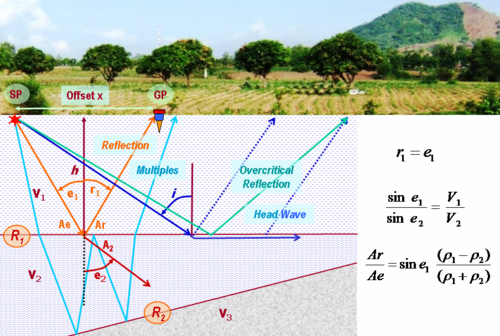
\includegraphics[scale=1]{figures/seismic_reflection_principal.png}
\caption{Seismic Reflection Outlines\cite{seisreflection}}
\label{seismic_reflection}
\end{figure}

%A landscape figure should be shown below. 
%%%%%%%%%%%%%%%%%%%%%%%%%%%%%%%%%%%%%%%%%%%%%%%%%%%%%%
%\begin{sidewaysfigure}[H]
%\centering
%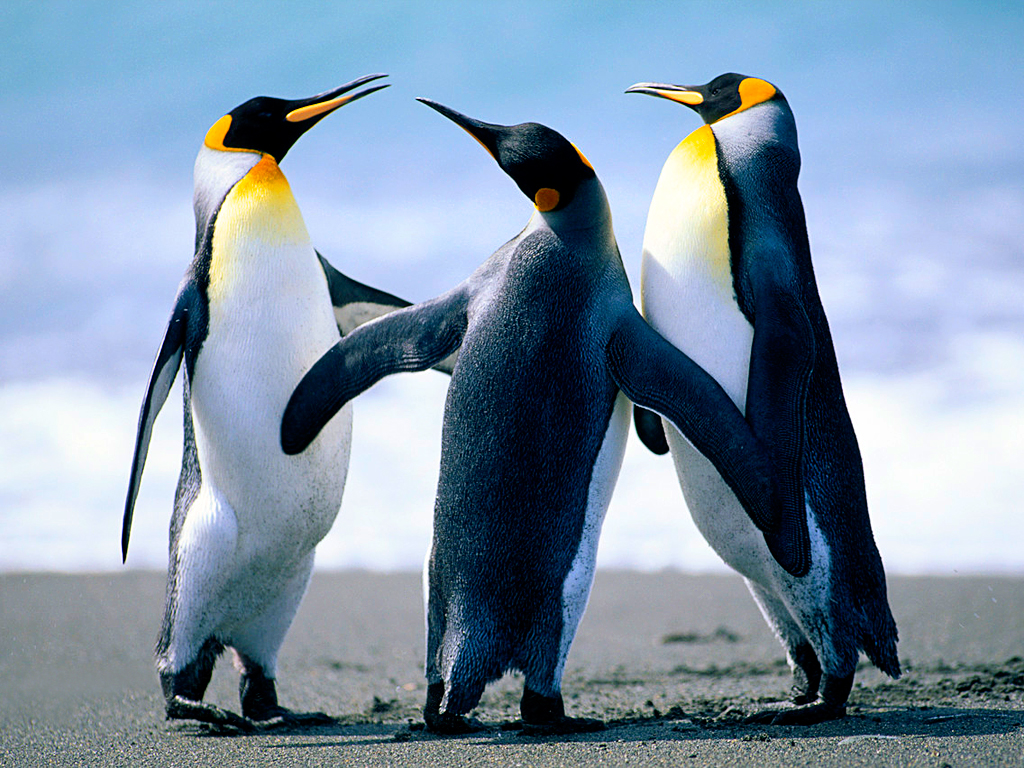
\includegraphics[scale=.50]{figures/Penguins.jpg}
%\caption{TAMU figure - This is an example of a long figure title with a landscape figure.  Figure titles need to be single-spaced within and double spaced between in the list of figures.}
%\label{fig:tamu-fig1-1}
%\end{sidewaysfigure}
%%%%%%%%%%%%%%%%%%%%%%%%%%%%%%%%%%%%%%%%%%%%%%%%%%%%%%


\section{Current Processing Methodlogy}
HPC technology has been used to process seismic data for several decades. In most current big oil \& gas companies or related service companies, there must have an IT department and a huge group of geophysicists or data scientists forming the research teams. In normal case, each small team set up a research project, and then develop new models or algorithms to verify their idea. In this stage, they only use synthetic or historical small data to do experiments, and their programming environment is MATLAB in general. But why did not they experimentalize on big cluster with actual seismic data? The main reason is that geophysicists are not familiar with HPC environment, and their main target is to verify the validity of algorithms or models, but not the performance. The volume size of actual data is usually very large and will take much more time to run with MATLAB codes. After research work was finished and got approval, geophysicists will submit their MATLAB codes to IT department, and then experts in HPC domain will translate such codes into MPI codes or hybrid OpenMP/MPI codes and verify them on high performance cluster with actual seismic data. If there are any problems in such stage, the original authors need to be involved to find the root cause together, and the results were either changing algorithms\/models by geophysicists or modification of programming implementation. To make such a research project become a mature product, it will often take one more year with several iterations.

%\subsection{This is a Very Long Subsection Title This is a Very Long Subsection Title}


\section{The Facing Challenges}

\subsection{Problems of Existing Solution}
In fact, there are problems in current seismic data analytics flow. As shown in previous section, the MATLAB codes work well on sample data do not mean they could run successfully in parallel after translating into MPI codes. The test cases on MATLAB codes are usually not enough, and the parallization itself may also produce new problems.
Another problem is the maintainence and reuse of legacy codes; Most of HPC codes in such area were written in Fortran to achieve high performance, the readability and maintenance of such programs are also challeges for beginners or successors. With the improvement of CPU computation power and programming architecture, we should not only focus on executation time, but also the overall performance of whole company and entire industry. 

\subsection{New Challenge from Big Data}
Currently, almost every industry could not live without network. With network including Internet, the data scattered everywhere could be transfered and be integrated for processing and analysis, and then form the basis for some new business such as search engine, social network and E-commerce etc. With the boom of social network, everyone becomes a media source intead of traditional centialized media portal, and the transaction data of online shopping increase drastically in recent years. Besides these popular area, some new direction such Internet of Thing (IoT) also grows quickly, so the big data has already been generated and will continue increase exponentially, which is big challenge for every industry.    

Big data\cite{WikiBigData} is a broad term for data sets with large volume,complext variety and high velocity which could not be handled by traditional data processing applications. The biggest challenges in seismic domain from now on are burst increase of acquired data volume size and high-speed streaming data from sensors in well need to be analyzed on time. Conventional RDBMS could not store wide variety data obviously, and moreover, different types of data from exploration, simulation and well logs need to be analyzed jointly, which also need more advance algorithms and models to process. For instance, the volume size of high dimension such as 3D even 4D seismic data and high density seismic data are growing exponentially, so seismic data processing becomes both computation- and data- intensive problems. The traditional HPC programming model is good at handle computation intense case, but for huge increase of volume size, data movement between nodes is the greatest bottleneck even with infiniband connections. In summary, oil \& gas domain also facing the big challenges including data storage, transfer, analysis and visualization etc.


%%%%%%%%%%%%%%%%%%%%%%%%%%%%%%%%%%%%%%%%%%%%%%%%%%%
%
%  New template code for TAMU Theses and Dissertations starting Fall 2012.  
%  For more info about this template or the 
%  TAMU LaTeX User's Group, see http://www.howdy.me/.
%
%  Author: Wendy Lynn Turner 
%	 Version 1.0 
%  Last updated 8/5/2012
%
%%%%%%%%%%%%%%%%%%%%%%%%%%%%%%%%%%%%%%%%%%%%%%%%%%%
%%%%%%%%%%%%%%%%%%%%%%%%%%%%%%%%%%%%%%%%%%%%%%%%%%%%%%%%%%%%%%%%%%%%%%
%%                           SECTION III
%%%%%%%%%%%%%%%%%%%%%%%%%%%%%%%%%%%%%%%%%%%%%%%%%%%%%%%%%%%%%%%%%%%%%

\chapter{\uppercase{Related Work and State of Art}}

There are so many research scientists working in large oil \& gas companies and related service companies, but in such a mature industry, it is very difficult to find complete open source codes or complete sample data on Internet. The main reason should be Intellectual Property issue; In the last twenty years, the oil \& gas becomes the most profitable industry. As there is less unexplored area, how to find the valuable oilfield is the most important task for oil \& gas companies. With the intensifying competition, the exploration data became very expensive and every company either kept its technology secret or applied for patents to protect itself.    

In normal case of seismic data processing, most companies will both write their own algorithms and use commerical softwares such as MATLAB, Petrel from Schlumberger, Paradigm software suite etc. The previous ones are mostly used to verify and its own customized algorithms or models that could be optimized basing on requirement, on the other hand, commercial softwares are mainly used in imaging and interpretation stages. But most of them could only run on single node, the performance is critical problem while handling big data.  

\section{Classical Open Source Seismic Softwares}
Besides commerical softwares, there is a list of free geophysics softwares in \cite{listofgeosw}. Among them the most famous one is Seismic Unix (SU) \cite{SUHome}. SU provides a series of tools for seismic data processing, such as data loading and storing data to and from files, data format conversion, transformation and filtering, processing utilities including stacking data, velocity analysis and migration etc. \cite{SUManual}. SEPlib \cite{SEPlibHome} contains programs to manipulate and process many types of geophysical data. It introduces two principles: Separate the geometry information from the seismic data, and exploit as much as possible the existing regularity in the data geometry, thus enable users and programmers to deal with irregularly sampled data with the same simplicity and efficiency \cite{SEPManual}. Madagascar \cite{MadagascarHome} is a moden package that provides a powerful environment for multidimensional data analysis and a convenient project management system. It provides two main ways of running application: shell scripts that use piping mode to run programm similiar to seismic unix, and Python scripts using SCons. Comparing with SU, Madagascar provide more programms and an open platform that support multi-language (C,Python and Fortran 90) on which user could add his own programms and share with others. The Mines Java Toolkit (JTK) \cite{JTKHome} is a set of Java packages and native (non-Java) code libraries for science and engineering including digital signal processing and 2-D and 3-D graphics. OpenSeaSeis \cite{OpenSeaSeis} is a sequential trace flow system that uses standard I\/O for passing traces from module to module as SU and provides a base system for managing the trace flow. OpendTect \cite{OpendTectMainPage} is a seismic post-processing and interpretation system, as well as an R\&D platform, for developing innovative seismic interpretation tools.

There are also some MATLAB libraries mainly used for research; CREWES Matlab Toolbox \cite{CREWESMatlab} is a very large collection of geophysical routines used in signal processing, wave propagation, velocity and migration methods etc. S3I \cite{CeGPS3I} provides an easy MATLAB-based library to simulate seismic imaging, which could also produce synthesized data basing on given velocity model, providing a platform for processing pipeline in seismic imaging and building features for interpretation and reservoir modeling.  

\begin{figure}[h]
\centering
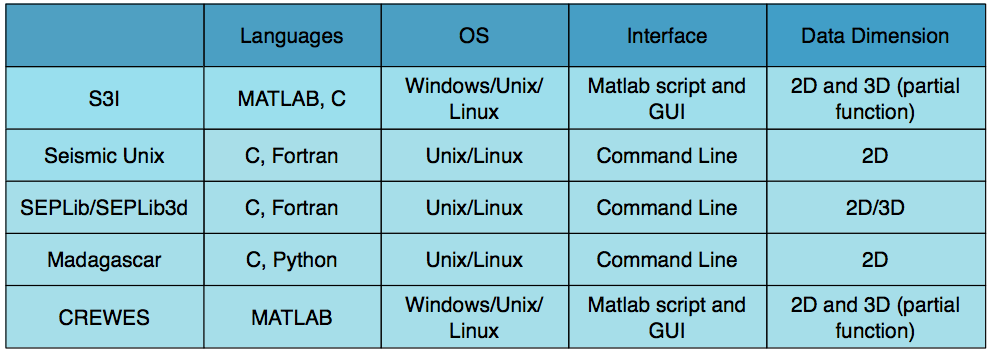
\includegraphics[scale=.42]{figures/open_package_list.png}
\caption{Comparison of open source packages \cite{CeGPS3I}}
\label{open_package_list}
\end{figure}

\section{Handle the Big Data}
Actually, all open source seismic softwares discussed in previous section are only used in research area. Not to say performance of MATLAB codes, all of these packages are sequential codes that could not run in parallel, so it is impossible for a company using such softwares in commerial purpose. As discussed in privious charpter, even the popular used HPC technology could not handle big data problems. 

Big data distinguish itself from traditional data in three main characteristics: volume, variety and velocity \cite{CharactOfBigData}. The increasing of volume size make it impossible to store and process data in single node, which is a big challenge to existing storage solution and computation model. Variety means data may come from different sources with different types, so the available RDBMS could not handle it, and how to store data efficiently and how to retrieve useful data for analysis are main problems to solve. As for the high velocity, which means large data are generated in real time environment and need to be analyzed on time due to the lifetime of data utility \cite{CharactOfBigData}, it also involves data storage and processing model issues. Through research and pratice in last decade, there are already several common open platforms that could handle big data effectively. In \cite{ChallengeOfBigData}, the author groups big data technologies into two categories, big data processing and big data persistence. Basing on data source and timeliness requirement, there are three main data processing platforms: batching processing, streaming processing and fast\/real-time processing. Distributed file system that could handle big data and NoSQL(Not Only SQL) that focus on unstructured data are main solutions in big data persistence, and the target of them are provide both high-availability and scalability to processing application.  

\subsection{Batch Processing Platform}
Google first released two papers on GFS(Google File System) in \cite{GhemawatGFS945450} and MapReduce in \cite{DeanMSD1251264} at 2004, which had been used by Google for storing and analyzing web search data. Basing on such ideas, Apache proposed open source implementation named Hadoop \cite{ApacheHadoop}. Hadoop provides big data storage solution with HDFS and big data processing modle with MapReduce. There are a lot of software packages built on Haoop, such as HBase \cite{ApacheHBase}, Hive \cite{ApacheHive} and Pig \cite{ApachePig} etc., which make Hadoop become the most popular ecosystem on big data batch processing. In \cite{2432874MohammadzaheriDISRAYMapReduce}, \cite{6118958RizvandiMapRecudePKTM} and \cite{2745578AddairSeismicSignalHadoop}, some traditional signal processing and migration algorithms are already implemented on MapReduce platform. \cite{6427595WangMultimediaMapReduce} built a large scale multimedia data mining platform by using MapReduce framework, where the processing dataset is similar to seismic image. However,  MapReduce only supports batch processing and relies on HDFS for data distribution and synchronization, which have significant overheads for iterative algorithms. Furthermore, there is no support for streaming and interactive processing in MapReduce, which becomes the biggest hole for supporting time sensitive data processing applications.

\subsection{Streaming Processing Platform}
Storm \cite{ApacheStorm} originally conceived and built by the team at Twitter to analyze the tweet stream in real time. The goal of Storm is to make it easy to write and scale complex real time computations on a cluster of computers. Storm guarantees that every message will be processed, and it is able to process millions of tweet messages per second with a small cluster. 
Storm YARN enables Storm applications to utilize the computational resources in a Hadoop cluster along with accessing Hadoop storage resources such as HBase \cite{ApacheHBase} and HDFS. Although it is scalable to process streaming messages, Storm is not designed for batch and interactive execution, and mostly focuses on text based message processing. 

\subsection{In-Memory Hybrid Platform}
To reduce the overhead of shuffling data into HDFS and to support more widely used iterative algorithms, there raised several in-memory computing frameworks. Apache Flink \cite{ApacheFlink} is a fast and reliable large-scale data processing engine, which is originally coming from Stratosphere \cite{Alexandrov2013Stratosphere}. It provides in-memory data sets, query language, machine learning algorithms and interfaces handling streaming data. Besides providing batch processing function, Flink is good at incremental iterations by pipelining data in an execution engine, which makes it suitable for most machine learning algorithms. 
Spark \cite{ZahariaSCC1863113} is a quick-rising star in big data processing systems, which combines the batch, interactive and streaming \cite{ZahariaDSE2342773} processing models into a single computing engine. It provides a highly scalable, memory-efficient, in-memory computing, real-time streaming-capable big data processing engine for high-volume, high-velocity and high-variety data. Moreover, it supports high-level language Scala that combines both object-oriented programming and functional programming into a single programming model. The innovative designed Resilient Distributed Dataset (RDD) \cite{SparkRDD} and its parallel operations provide a scalable and extensible internal data structure to enable in-memory computing and fault tolerance. There is a very active, and fast-growing research and industry community that builds their big data analytics projects on top of Spark. 
Apache Ignite \cite{ApacheIgnite} In-Memory Data Fabric is a high-performance, integrated and distributed in-memory platform for computing and transacting on large-scale data sets in real-time, orders of magnitude faster than possible with traditional disk- or flash-based technologies. 
However, all these frameworks are built for general propose cases and are focused on data parallelism with improved MapReduce model, and there is no communication mechanism between workers, which does not fit to some iterative seismic algorithms requiring frequent data communication among workers. The global memory technique could be achieved by adding communication layers to existing platforms or by storing data into database. 

\section{Big Data Persistence and Data Locality}
With the growing exponentially of the seismic data volumes, how to store and manage the seismic data becomes a very challenge problem. The legacy HPC computing model needs to distribute data to every worker node, which will consume more time on data transferring. The trend toward big data is leading to transitions in the computing paradigm, and in particular to the notion of moving computation to data, also called near-data-processing(NDP) \cite{6871738BalasubramonianNDP}. In Data Parallel System such MapRecuce \cite{6217449GuoDataLocalityMapReduce}, clusters are built with commodity hardware and each node takes the roles of both computation and storage, which makes it possible to bring computation to data. In \cite{6267846PerroneReducingDataMovement}, it presented an optimized implementation of RTM by experiments with different data partitioning, keeping data locality, and reducing data movement. In \cite{NextDataCenterVisualization}, it proposed a remote visualization solution by introducing GPU computing into cluster, which could overcome problems of dataset size by reducing data movements to local desktop. In \cite{6092321VoParaVisMapReduce}, it evaluated the suitability of MapReduce framework to implement large-scale visualization techniques by combining data manipulation and data visualization system on cluster. 

Besides  binary seismic data, there are huge amount semi-structured data and metadata generated at seismic data acquisition and processing. There are some obvious limitations of traditional RDBMS to handle this kind of big data; RDBMS is not flexible to handle different types of data, and there are also scalability and performance limitations on RDBMS. The NoSQL database is designed to be more suitable in such a scenario. HBase \cite{ApacheHBase} is a distributed, scalable and column\-based database after Google's Bigtable \cite{BigTableChang1365816} which is good at random, realtime read/write access to big data. Cassandra \cite{ApacheCassandra} is a distributed NoSQL database designed to handle large amount of data that could achieve linear scalability and fault-tolerant ability without compromising performance. MongoDB \cite{MongoDBNoSQL} is a document-oriented NoSQL database that casts focus on flexible data model and highly scalability. Redis \cite{RedisNoSQL} is a data structure server that provides key-value cache and storage, and it works with in-memory dataset thus could achieve outstanding performance. Based on the characteristics of seismic data, Cassandra could be used to save metadata and provide dataset to Spark, while Redis could be used to store intermediate data shared by all workers.Inspired by Google’s Dremel, Apache Drill \cite{ApacheDrillMain} is a low latency distributed query engine for large-scale datasets, including structured and semi\-structured/nested data. 

\section{New Algorithms\&Models Applied on Seismic Data}
With the increasing volume size of seismic data, the algorithms applied on data also become more sophisticated to extract valuable information. Some advanced machine learning algorithms are already used in this area. \cite{7067356ChakiPredictSandNeuralNetwork} used artificial neural network (ANN) to predict sand fraction from learning multiple seismic attributes such as seismic impedance, amplitude, and frequency. In \cite{6234749DengSVMPredictReservoir}, it set up a model by feeding five seismic attributes and the reservoir thickness to train Support Vector Machines (SVM) and then used it to predict the reservoir thickness. \cite{4026836MachadoNerualNetworksFault} used meta-attributes to train multi-layer neural networks and evaluated the effectiveness of the new generated seismic fault attribute. \cite{6707117KaurPWaveANN} used Back Propagation Neural Network (BPNN) for the automatic detection and identification of local and regional seismic P-Waves. 
Petuum \cite{Dai2013Petuum} is distributed machine learning framework that is focused on running generic machine learning algorithms on big data sets and simplifying the distributed implementation of programs. Based on characteristics of machine learning algorithms, Petuum provides iterative-convergent solutions that quickly minimize the loss function in a large-scale distributed cluster. Since these frameworks such as Petuum and Graphlab \cite{DatoGraphLab} are designed specially for machine learning algorithms, they could get better performance comparing with other general purpose MapReduce frameworks that emphasize on consistency, reliability and fault tolerance. 

In summary, traditional open source seismic package clould only handle small volume size seismic data, and although there are already many research projects trying to solve the big data problem, but there is still no perfect solution designed specific to seismic data. The MapReduce platform and its predecessors are too common to support complicate seismic algorithms, while some other platforms either emphasize on performance of computation or model optimization in narrow specific area. All existing opensource seismic packages are not friendly for domain-specific experts.
To make it easy for geophysicists and data scientists processing and analyzing big seismic data, a new platform is needed by incorporating the advances of big data research into the industry. Such a platform should not only be capable of processing big data efficiently and running advanced analytics algorithms, but also should achieve high usability, fault tolerance and good scalability. Data management and distribution supporting both structured and unstructured need to be hiden in order to allow geophysicists to utilize the platform easily. Moreover, typical seismic analytics algorithm templates and workflow would be very useful to simplify their work and to improve overall performance. 


%%%%%%%%%%%%%%%%%%%%%%%%%%%%%%%%%%%%%%%%%%%%%%%%%%%%%%%
%\subsection{Subsection}

%A table example is going to follow.

%\begin{table}[H]
%\centering
%\caption{This is a table template}
%\begin{tabular}{|l|c|c|c|c|c|}
%\hline
%Product & 1 & 2 & 3 & 4 & 5\\
%\hline
%Price & 124.- & 136.- & 85.- & 156.- & 23.-\\
%Guarantee [years] & 1 & 2 & - & 3 & 1\\
%Rating & 89\% & 84\% & 51\% & & 45\%\\
%\hline
%\hline
%Recommended & yes & yes & no & no & no\\
%\hline
%\end{tabular}
%\label{tab:template2}
%\end{table}
%\subsubsection{This is a subsubsection}



%%%%%%%%%%%%%%%%%%%%%%%%%%%%%%%%%%%%%%%%%%%%%%%%%%
%
%  New template code for TAMU Theses and Dissertations starting Fall 2012.  
%  For more info about this template or the 
%  TAMU LaTeX User's Group, see http://www.howdy.me/.
%
%  Author: Wendy Lynn Turner 
%	 Version 1.0 
%  Last updated 8/5/2012
%
%%%%%%%%%%%%%%%%%%%%%%%%%%%%%%%%%%%%%%%%%%%%%%%%%%%
%%%%%%%%%%%%%%%%%%%%%%%%%%%%%%%%%%%%%%%%%%%%%%%%%%%%%%%%%%%%%%%%%%%%%%
%%                           SECTION IV
%%%%%%%%%%%%%%%%%%%%%%%%%%%%%%%%%%%%%%%%%%%%%%%%%%%%%%%%%%%%%%%%%%%%%

\chapter{\uppercase{Implementation of Seismic Analytics Cloud Platform}}
To solve the problems stated in previous chapters, we develop seismic analytics cloud platform (SAC for short). The goal of SAC is to deliver a scalable and productive cloud Platform as a Service (PaaS) to seismic data analysis researchers and developers. SAC has two main characteristics: one is able to process big data and another is easy to use for geology domain experts. With SAC, user only need focus on data analytics logic itself without caring about details on data storage and computing model. 

%SAC is designed to be able to store large amount of seismic data with major vendor's formats, as well as be able to process them in the scalable fashion to meet the performance requirements. Users should be able to work on their seismic processing algorithms using high-level programming models with very limited knowledge in parallelism and architecture.

\section{Architecture of SAC}

In the beginning, the mainframe is widely used for seismic data processing and each job regardless of running time needs to be put into queue waiting for execution. With the improvement of CPU power, more softwares were transferred to personal computer(PC) for better portability and interactivity. But with the growth volume size of seismic data, frequency of single core could not increase limitless and scalable resources are need to handle variable requirements, more and more softwares are then moved to cloud platform by utilizing parallelization dynamically. Such trend brings big change on business model: from selling software license to charging for service. In cloud platform, the thin client could request storage and computation resources basing on requirement, and in such way whole cluster or huge data center could be used efficiently. In HPC domain, MPI or PVM could also build on cluster, which fully utilize all resources in whole cluster but need deep understanding of data distribution and communication. The data storage in HPC is typical using centralized storage manager with disk array, which needs data movement between storage nodes and worker nodes. To overcome problems of HPC, we build SAC as service with template-based programming interface on cloud platform, and to make it easy to use, some popular image processing and signal processing software packages are integrated into SAC.  


Figure \ref{SACSWStack} shows the overall software stack used in SAC. In this diagram, the operating systems at 1st level from bottom to top could be Unix-like or Windows system running on virtual machine or bare metal. Above the OS layer, there should be a layer provides compiling and running environment, which include JRE/JDK, Scala, Python and other native libraries such as OpenCV \cite{OpenCVMain}, FFTW \cite{Frigo05thedesign} etc. Java has already became the dominating language in application development for its cross-platform and simplicity \cite{Top10Lang}. Scala is a new general-purpose programming language that support both object-oriented and functional programming language but still runs on JVM and is compatible with existing Java libraries. Most big data processing platform such as Hadoop, Storm, HBase and Cassandra etc. are written in Java and provide Java programming interfaces; Spark is developed in Scala itself but applications running on it could be developed in Java, Scala or Python. For the performance issue, some computation intense libraries such FFTW and OpenCV are written in C++, but they also provide Java interface through JNI that could be used on JVM. In third layer, there are some common componets installed including HDFS, Mesos \cite{ApacheMesos} and YARN \cite{ApacheHadoop}  used for data storage and resource scheduling. HDFS is distributed file system delivered in Hadoop that provides highly fault-tolerance and high throughput access to big data set. In SAC, HDFS is used for storing original binary seismic data. The metadata and intermediate data such as seismic attribute are stored in Cassandra database. Resource management in cluster is very important for job scheduling and load balance, and in SAC, Standalone, Mesos and YARN are all supported. In the fourth layer from bottom, it includes the actual computation components: signal and image processing libraries with Java/Scala interface; Breeze \cite{ScalaNLPBreeze} is a set of libraries for machine learning and numerical computing written in Scala and Java. FFTW is a C subroutine library for computing the discrete Fourier transform (DFT) with one or more dimensions in both real and complex data format. There are already some Java FFTW wrappers make it could be used on JVM without giving up performance. SAC chose Spark as computation platform due to its performance achieved with in-memory computation and its fault tolerance. The main work of this paper are focus on second and third layer from top. Seismic Analytics Cloud layer is used for providing SDK and running environment for client applications.SAC Framework plays most important role in this cloud platform, and it is the bridge of user's application and running environment on cluster. Template-Based framework provides common programming models for domain specific experts, and workflow could connect piece of algorithms or models into a job chain as well as run it automatically. Visualization is important for user to view results and generate useful information intuitively. Seismic Applications on the top of stack are mainly developed by end users. There is a user friendly web interface provided to user, on which user could view datasets, programming and testing single algorithm or running workflow in convenient way by drag-and-drop of widgets. Some other issues should also be considered on cloud platform, such as data security, job scheduling and resource sharing etc.   

%The design of SAC architecture is to emphasize twofold: one is to provide a high-level productive programming interface to simplify the programming efforts; the other is to execute user's applications with scalable performance. To achieve the first goal, we provide the web interface in which user could manage seismic datasets, programming within a variety of templates, generate complete source codes, compiling and then running the application and monitoring the job running status in SAC. 

%The interface allows users to write seismic data processing algorithms using our extracted common seismic computation templates, which lets users focus on their kernel algorithm implementation, and simplifies user's implementation in handling seismic data distribution and parallelism. While the most popular-used programming models in seismic data processing include MATLAB, Python, C/C++, Fortran, Java and more, SAC supports Java, Python and Scala natively, so that users can write their own processing algorithms directly on our platform with these three languages; For legacy applications written in other languages, SAC uses the so-called PIPE mode to handle input and output data as standard-in and -out, which requires minor modifications of program source code on handling input and output. SAC will generate complete Spark codes based on user's kernel codes and configurations, and then launch and monitor it on the SAC environment. In order to support large amount data storage and scalable I/O performance, we chose Hadoop HDFS as the underlying file system, which provides fault tolerance with duplicated copies and good I/O throughput by supporting data locality information to applications. HDFS supplies out-of-the-box redundancy, failover capabilities, big data storage and portability. Since the size of seismic data is very large and keeps increasing constantly, HDFS provides a good solution for the data storage with fault tolerance property.

%We use Spark as the parallel execution engine to start applications, since Spark works well on top of HDFS, Mesos [13] and YARN, and it provides a big data analytics computing framework with both in-memory and fault-tolerance support. Spark provides RDD \cite{SparkRDD} as a distributed memory abstraction that lets programmers perform in-memory computations on large-scale cluster/cloud in a fault-tolerant manner. To get better performance, we need to put frequently used data into memory and processing data in memory, which is one key performance boost comparing with MapReduce.Some other useful packages and algorithms in data analytics, such as SQL, machine learning and graph processing, are also provided in Spark distribution version. We also integrated some common used libraries for image processing and signal processing, such as OpenCV, Breeze and FFTW etc., to provide a rich third party of libraries support to speed up the development process. Figure \ref{SACSWStack} shows the overall software stack used in SAC.

%Figure \ref{SACArch} presents the overall architecture of SAC. Based on the SAC web interface, Users are able to upload, view and manage their seismic data, which are stored on HDFS. They can then create their application projects by selecting a template from a list of predefined templates to start their own programming. After selected dataset and processing pattern, writing codes and compiling successfully, users can configure the running parameters and then submit jobs to SAC. Job status could be monitored while job is running and running results could be checked after job is finished. On the SAC backend, a big seismic data file will be split into multi-partitions and be constructed into RDD, which will be processed by working threads that apply user's algorithm in parallel. After all data are processed, the output data will be saved back to HDFS.

Figure \ref{SACArch} shows the overall architecture of SAC, in which there are three main parts: data flow, operations on data and user interface.
The upper part of such diagram shows a complete processing lifecycle of seismic data on SAC; At first, seismic data need to be uploaded to HDFS. In the view of end user, it is still a big file, but HDFS will store it on different nodes block by block. User could also preprocess and view data as needed. To make such a huge file be processed by multi-nodes, it will be split into small partitions and then user's transformations could be applied on them. When all operations on each partition finished, user could run some actions to persist results. Such results could be used for further processing, visualization or statistics etc.  

%%%%%%%%%%%%%%%%%%%%%%%%%%%%%%%%%%%%%%%%%%%%%%%%%%%%%%
\begin{figure}[h]
\centering
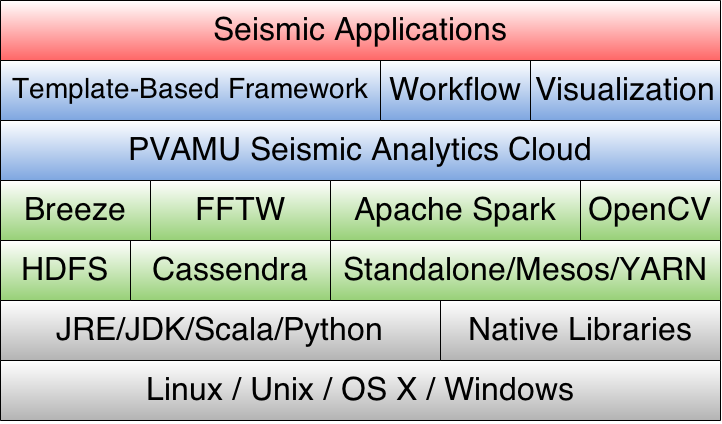
\includegraphics[scale=.50]{figures/SACSWStack.png}
\caption{The Software Stack of Seismic Analytics Cloud Platform}
\label{SACSWStack}
\end{figure}
%%%%%%%%%%%%%%%%%%%%%%%%%%%%%%%%%%%%%%%%%%%%%%%%%%%%%%

%%%%%%%%%%%%%%%%%%%%%%%%%%%%%%%%%%%%%%%%%%%%%%%%%%%%%%%
\begin{figure}[h]
\centering
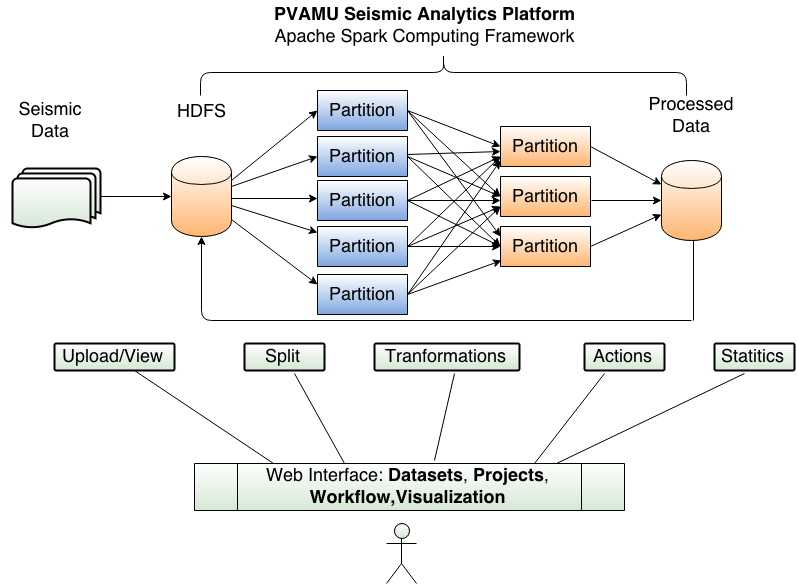
\includegraphics[scale=.50]{figures/SACArch.png}
\caption{The Architecture of Seismic Analytics Cloud Platform}
\label{SACArch}
\end{figure}
%%%%%%%%%%%%%%%%%%%%%%%%%%%%%%%%%%%%%%%%%%%%%%%%%%%%%%%

\section{Data Storage and Distribution}

There are many file formats used for storing seismic data, such as SEGY \cite{SEGYREV1}, SEGD \cite{SEGDREV21}, SEED \cite{IRISSEED} etc. Some popular softwares even have their own intermediate formats to make it easy for processing; Sesimic Unix has SU file format, OpendTect \cite{OpendTectMainPage} use CBVS(Common Binary Volume Storage) format, and SEPlib has its own SEP3D file format that separate ASCII metadata with actual binary trace data. In current stage, only widely used SEGY file format is supported in SAC. Other data formats could be easily added in data preprocess stage.
The SEGY (also SEG-Y) \cite{SEGYREV1} file format is one of several standards developed by the Society of Exploration Geophysicists (SEG) for storing geophysical data. It consists of 3200 bytes textual file header, 400 bytes binary file header and trace data. Each trace has a 240 bytes header and variable binary trace data. In normal case, application need to parse file header to get some useful information about survey at first, then get a 2D/3D volume for further processing. To process SEGY file in parallel, such big seismic data needs to be split into multiple small partitions. The SEGY file could not be split directly: every worker node need to access header description information, and not all traces have same size of data. Meanwhile, most algorithms need to use one complete trace or plane as input, so one trace or one line could span more than two splits.   

So we introduce a preprocess program, transferring SEGY file into two files: one is xml file used to describe metadata, another file saves all traces data with equal size after interpolation. There are two pros with this format: xml file sharing same trace data file could save some other job related information about how to split trace data, and only xml files needs to be changed in most cases; trace data file could be split easily on requirement. Hadoop use InputFormat to split data, Which is also supported by Spark. The default InputFormat classes could not handle text file and binary file together, so we implemented a new SeismicInputFormat class in SAC. SeismicInputFormat use xml file as input, trying to parsing information from it and generate split list. Spark driver will send split to each executor, and then each task in executor will call SeismicRecordReader get trace data from file on HDFS. After Spark load seismic data from HDFS, it will generate an in-memory RDD for improving performance. The basic information about survey such as location of related trace data file, dimension, data type information are store in xml file, and beside those, user cloud also define other parameters used for application running. When user create a new project, he could define how many lines each split and number of overlap lines, and such parameters determine the offset and size of each split. As a rule, the seismic data is stored trace by trace in Inline direction, but there may be some algorithms need to process data in cross-line for time-depth direction. Such direction could also be defined in xml file, and SAC will load data in Inline direction into memory and then make in-memory transformation to generate a new direction RDD.
  
%However, SEGY data could not be split directly due to its irregularity, so we preprocess the SEG Y data format into a regular 3D volume data, and store the important header information into one xml file. Then the 3D volume data and xml will be feed into Spark applications. Spark uses InputFormat, which is the base class inherited from Hadoop to split such data and construct RDD. Each split will be mapped to one partition in RDD. The embedded InputFormat classes could not handle binary seismic data, so we implemented SeismicInputFormat in this project.  Based on configuration defined by user while creating project, such as how many lines each split and number of overlap lines, SeismicInputFormat could spilt the 3D volume and feed partition to each mapper. The data of 3D volume is stored trace by trace in the Inline direction by default. For some algorithms that need to process data in cross-line or time-depth direction, we also provide interfaces to transform Inline format RDD into cross-line or time-depth direction. In this way, we could cache Inline format RDD in memory, thus all the transformations could be executed in memory with better performance.

%\begin{table}[H]
%\centering
%\caption{This is a table template}
%\begin{tabular}{|l|c|c|c|c|c|}
%\hline
%Product & 1 & 2 & 3 & 4 & 5\\
%\hline
%Price & 124.- & 136.- & 85.- & 156.- & 23.-\\
%Guarantee [years] & 1 & 2 & - & 3 & 1\\
%Rating & 89\% & 84\% & 51\% & & 45\%\\
%\hline
%\hline
%Recommended & yes & yes & no & no & no\\
%\hline
%\end{tabular}
%\label{tab:template2}
%\end{table}

\section{Seismic RDD}
Resilient Distributed Datasets (RDDs) \cite{SparkRDD} is core concept proposed by Spark, which is a fault-tolerant collection of elements that can be operated on in parallel. RDDs \cite{ApacheSparkPG} support two types of operations: transformations, which create a new dataset from an existing one, and actions, which return a value to the driver program after running a computation on the dataset. Even in parallel programming on cluster, the program still consists of data structure and algorithms. Spark uses the RDD as a common data structure that distributed in multi-nodes, and provides some typical operations as algorithm frameworks in functional language style so that user could plug in his own algorithms and apply them on RDD. Comparing with traditional parallel programming model such as MPI and OpenMP, the programming on Spark is much simpler. But for geophysicists or data scientists who have no much idea about RDD and functional language, there are still some tedious works to do. SAC tried to simplify work by introducing Seismic RDD and Template. User only need configure some parameters: The dataset need to process, input and output type of algorithms, then write a piece of codes, SAC will generate Seismic RDD, create template, merge user's codes and run them automatically. Seismic RDD is built from SeismicInputFormat, and besides the basic operations provided by Spark, Seismic RDD also provide some other features: fine-grain function on pixel or trace inside each split, transferring RDD from default inline direction to other directions automatically basing on configuration, override some operators for easily used by high level applications. The most advantage of RDD is caching most frequently used data in memory, thus improving performance of some iteration algorithms drastically. In normal case, the RDD is only valid within the lifetime of SparkContext, so RDD in memory will be discarded after application finished. Spark-jobserver \cite{SparkJobserver} provides a RESTful interface for submitting and managing Apache Spark jobs, jars, and job contexts, and moreover it introduces the concept of Named RDDs. With Named RDDs, several applications or jobs sharing the same context could cache and retrieve RDDs by name, thus improve RDD sharing and reuse among jobs. In workflow component of SAC, several jobs in one workflow will use Named RDDs to avoid loading and releasing RDD frequently in each job.

\section{Template}

%Based on the general parallel execution patterns of seismic processing algorithms and applications, we predefined some templates to make this framework easy to program. Every template has explicit input type and output type. The typical templates are: Pixel pattern, which use sub-volume or one pixel as input and output one pixel; Line pattern, which treat one line as input and one line as output; SubVolume pattern, which feed user’s application with sub-volume and get output from it in sub-volume format. A high level SeismicVolume class has been implemented in this project to provide user interface to access seismic volume. SeismicVolume class provides functions for constructing RDD based on processing templates user had selected, applying user's algorithms on RDD, and storing the final RDD on HDFS with format defined by user. To make it easy for programming, we provide some other functions to change the linear array into 2D matrix and 3D volume class; some functional programming interface such as iteration, map/flatMap, filter and zip could be used. We also integrated commonly used high-level algorithms, such as histogram, FFT, interpolating and filtering algorithms, so that user could put more attention on data analytics logic instead of details for each algorithm.

Essentially, seismic data is a 2D plane or 3D volume composed by traces. The data type of trace data is Float type with IEEE floating-point format or IBM floating-point format. Classical signal processing or image processing algorithms have been widely used for processing seismic data. The grain size of input/output data could be sample point, trace, 2D plane or 3D volume. The relationship between volume size of input and the other one of output is shown in Figure \ref{Template}, in which solid circle (input data) or hollow circle (output) indicates one point, one trace, one plane or even one volume. The relationship could be 1 to 1 (Figure \ref{Template} a), N to 1 (Figure \ref{Template} b) or 1 to N (Figure \ref{Template} c). In some case such as median filter, there is overlap between each input split, which could be treated as a special case of 1 to 1, but the edges need to considered in data distribution. After study of popular open source seismic data processing package, signal processing and image processing packages such as SU, Madagascar, JTK, Breeze, OpenCV, ImageMagick etc., we define some typical templates in SAC: Pixel pattern, which use sub-volume or one pixel as input and output one pixel; Trace Pattern, which use one trace or several traces as input and output one or more traces; Line pattern, which treat one line or more lines as input and one line or more lines as output; SubVolume pattern, which feed users�� application with sub-volume and get output from it in sub-volume format. These templates could handle most cases with one seismic data set, but it could not handle other cases with two seismic data sets as input because map/flatMap functions can only be applied on one RDD. For such case with two RDDs, we can merge them into one RDD with zip function, and then apply map/flatMap functions on combined RDD. 

Beside these transformations, there are still some other summary operations or actions in Spark such as count, stats or collect etc. Those functions have no definite template, but are very useful yet. So SAC provides a free template by passing RDD directly to user's application, so user could call any transformations and actions as required. So some sophisticated models that are difficult to split into subtasks or have multiform input or output, free template is also effective. 

%%%%%%%%%%%%%%%%%%%%%%%%%%%%%%%%%%%%%%%%%%%%%%%%%%%%%%%
\begin{figure}[h]
\centering
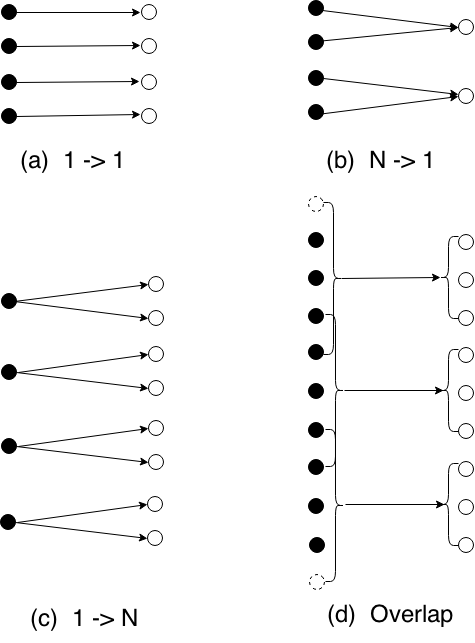
\includegraphics[scale=.50]{figures/template.png}
\caption{Relationship of Input and Output in Seismic Data Processing}
\label{Template}
\end{figure}
%%%%%%%%%%%%%%%%%%%%%%%%%%%%%%%%%%%%%%%%%%%%%%%%%%%%%%%

\section{Code Generator}

%After user created project and completed their own kernel codes, one component named Code Generator (CG) in SAC will generate complete Spark codes for running on Spark platform. The CG will parse configuration of user's project and generate Spark application outlined codes, merge them with user's codes. User could also upload existing source codes or libraries, all of which will be integrated into current working project managed by Simple Build Tool (SBT). CG will also generate compiling and running scripts basing on user's runtime setting. All these scripts will be called by the web interface, on which some other information such as compiling and running status, location of output will be shown clearly.

As explained in previous chapters, after generating a new project and finishing program by user, it is time to make it run. Code Generator (CG) in SAC will be in charge of such task: creating skeleton of project, generating template codes, setting up running time environments etc. Template was already discussed in previous section, and the main issue is definition of input type and output type. With such information, CG could generate outline of function to be completed by user. Basing on user's configuration, CG will also generate backend codes for loading data sets to RDD and saving output RDD back to HDFS or database. SAC uses Simple Build Tool (SBT) \cite{ScalaSBT} and Ant \cite{ApacheAnt} as project management tools. To make such codes run on Spark, CG generate source files list and dependencies list for SBT, then SBT will build all source codes and generate .jar file for current project. CG will also generate all runtime libraries list for Ant, and Ant will package all libraries into one .jar file for execution on Spark. CG will generate compiling script and running script too, which will be called by web interface.


\section{Application Execution}

%In SAC, every user's project will be treated as one Spark application. CG will generate the main driver code for each project. Each application could be submitted to SAC for running after compiled successfully. At execution time, driver code will setup the Spark running time environment, call the SeismicVolume object to generate RDD and execute user's algorithms on top of RDD and then store the processed results on HDFS. It will clean up the running environment and release resources after finished. To make it support multiple users, Spark Jobserver \cite{SparkJobserver}  was introduced to this platform. Based on the priority of application and computation resources requirement of an application, an user could configure the running parameters: number of cores and memory size; and then submit his/her own job, monitoring job status and viewing the running results. Another big advantage of Spark Jobserver is supporting of NamedRDD that allows multiple applications share RDD but has only one copy cached in memory. For some complicate algorithms that need multiple steps or application running in workflow, NamedRDD is a good choice for boosting performance. After job is finished, the running results cloud be discarded or be saved to user's workspace basing on user's selection.

As PaaS cloud platform, SAC provides two ways of executing application: running one job on Spark and running multi-jobs with workflow on Spark. To process big seismic data, each job may take much time, so on such a multi-user platform, job submission and job scheduling need to be planned carefully. To start a job, user need to configure how much resource it needs (memory, number of cores, scheduling policy) at first, and then submit job to Spark-jobserver. Once the runtime environment is satisfied, the driver code call the SeismicVolume object to generate RDD and apply user's algorithms on RDD and then store the processed results on HDFS or database. If there are any tasks failure at running time, Spark will only run the failed tasks basing on dependencies chain. All job status could be checked through web interface of SAC, and after job is finished, user could view results immediately through visualization component. For the workflow including multiple widgets, it need a driver to setup DAG at first and each widget is a independent job with clear-cut input and output at running time, but they could share save Named RDDs with same context for boosting performance.


\section{Application Programming Interface}
SAC itself is developed in Java/Scala language, so it could be compiled into jar library. User cloud call this library in his own application or use template and CG generate codes outline by filling algorithm snippet, but in both cases, user need to be familiar with API of SAC, configure application and control development procedure by himself. SAC also provides web interface to simplify installation of development environment on client side, in such case, user only need to select template, input codes snippet and then click buttons to compile, to run and to view results. 
When user want create a new algorithm or model, SAC will create a new project, in which user could select template, define data type of input and output, then SAC will generate function template for user to fill his own logic codes in it. SAC had integrated widely used libraries in seismic area such JTK, Breeze and OpenCV, so user could use them in programming or add his own libraries as requirement. After user finished coding, he could compile and run them immediately and view results after job finished. With web interface, user cloud also preview dataset, select data set as input for algorithm and check running result after job finished. Workflow is another big improvement for running batch jobs; Each long batch job are divided into small tasks, and each task is encapsulated as widget. User could select different widgets, configure parameter for each one and connect them into a long job, and then submit it to cluster. With workflow, the productivity, usability and flexibility are all improved. Currently, four main components on web interface: project coding and running, data set preview, job management and workflow. The web programs are written in PHP Language, JavaScript, HTML and CSS, while the workflow part are modified from Clowdflows \cite{ClowdflowsMain}. Some other popular web development components such as jQuery, bootstrap, user cake, dropzone, D3 and ace editor are used in web interface. To make SAC framework be used by web interface, a bunch of shell scripts are developed and are called by web interface. XML files are used for communication between web interface and SAC framework. The example XML file used to describe project is shown as below. 

\lstset{language=XML,frame=single}
\begin{lstlisting}[float,caption=Sample XML file of Project Configuration,label=XMLProjectConfig]
<?xml version="1.0"?>
<ProjectConfig>
  <user>pvamucloud</user>
  <rootDir>/home/cscloud/user/pvamucloud/Pixel</rootDir>
  <projectName>Pixel</projectName>
  <projectVersion>1.0</projectVersion>
  <unit>Pixel</unit>
  <inputType>Float</inputType>
  <outputType>Float</outputType>
  <direction>Inline</direction>
</ProjectConfig>
\end{lstlisting}

%%%%%%%%%%%%%%%%%%%%%%%%%%%%%%%%%%%%%%%%%%%%%%%%%%%
%
%  New template code for TAMU Theses and Dissertations starting Fall 2012.  
%  For more info about this template or the 
%  TAMU LaTeX User's Group, see http://www.howdy.me/.
%
%  Author: Wendy Lynn Turner 
%	 Version 1.0 
%  Last updated 8/5/2012
%
%%%%%%%%%%%%%%%%%%%%%%%%%%%%%%%%%%%%%%%%%%%%%%%%%%%
%%%%%%%%%%%%%%%%%%%%%%%%%%%%%%%%%%%%%%%%%%%%%%%%%%%%%%%%%%%%%%%%%%%%%%
%%                           SECTION V
%%%%%%%%%%%%%%%%%%%%%%%%%%%%%%%%%%%%%%%%%%%%%%%%%%%%%%%%%%%%%%%%%%%%%


\chapter{\uppercase{Experiments \& Results}}
To verify the idea proposed in this thesis, we setup experiment environments, develop SAC framework and run some typical seismic applications on cluster in PVAMU cloud computing lab. There are three main layers in SAC: low-level runtime environment, SAC framework as middleware and application development interface at up-level. Middleware layer of SAC was already discussed in pervious section. Runtime environments is the basic that SAC built on, and the application development interface is entry of user, which will be introduced respectively in the following sections.

\section{Experiments Environment Setup}

The cluster used for conducting experiments consists of 26 nodes, in which one is management node, another is storage node used for managing disk array and other 24 nodes are computation nodes. Each node in such cluster was equipped with Intel Xeon E5-2640 Sandy Bridge CPU (2.5GHz, 12 Cores or 24 Cores with Hyperthreading support), 64GB DDR3 memory and are inter-connected with 1GB ethernet. Each node has its own local disk, and also could access disk array through NFS. Following the architecture stated in previous charpter, we install CentOS 6.5 (Distributed by Redhat) and Oracle JDK 1.8.0\_40 on each node. Hadoop 2.2.0, Spark 1.2.1 (update to Spark 1.4.0 late) and other related libraries are also installed on each node. In configuration of Hadoop, management node was configured as NameNode and other 24 computation nodes as DataNodes. It is similiar in Spark: management node is Master and other computation nodes are Workers. Cassandra was installed on all 24 computation nodes and the first four nodes was selected as seed nodes.

The public sample seismic dataset Penobscot \cite{PenobscotData} was selected as experiment data. The original format of Penobscot dataset is SEGY, and to make it easily processed with Spark, we transfer it into two files: one xml file that saves meta data, and another 3D data file with dimension size of 600x481x1501 stores actual data samples. The volume size of original data file is about 1.7GB, which is not big enough comparing with data set currently used in oil\&gas industry, so we use it synthesize a new 100GB file for verifying algorithms and models on SAC. For some extensive time consuming algorithms, we still use 1.7GB file as test data. Both xml file and data file are stored on HDFS, so that every node could access them and utilize data locality. The intermediate results are stored in Cassandra basing on requirement and final result are persisted back to HDFS. 

\section{Application Development Platform}

As stated in previous charpter, user could create new application that calls APIs provided by SAC framework directly, but another more convenient way is using Web interface provide by SAC platform. In web development interface, SAC platform provides four main components: Projects, Data Sets, Jobs and Workflow. The typical flow is listed below:

\begin{enumerate}
  \item Create a project or open an existing project. While create new project, user need to select template as shown in Figure \ref{NewProject}.
  \item Edit codes, compile project and fix erros until compiling successfully as shown in Figure \ref{Programming}.
  \item Select data set(s) as input parameter as shown in Figure \ref{DataSet}.
  \item Configure runtime environments and submit job to Spark Jobserver as shown in Figure \ref{Runtime}.
  \item Check job status and view results after job finished.
\end{enumerate}

%%%%%%%%%%%%%%%%%%%%%%%%%%%%%%%%%%%%%%%%%%%%%%%%%%%%%%%
\begin{figure}[H]
%\centering
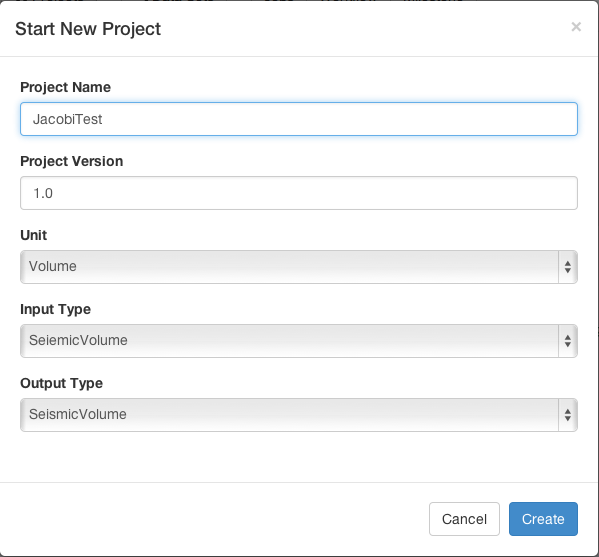
\includegraphics[scale=.60]{figures/NewProject.png}
\caption{Configure Template on Creating New Project}
\label{NewProject}
\end{figure}
%%%%%%%%%%%%%%%%%%%%%%%%%%%%%%%%%%%%%%%%%%%%%%%%%%%%%%%

%%%%%%%%%%%%%%%%%%%%%%%%%%%%%%%%%%%%%%%%%%%%%%%%%%%%%%%
\begin{figure}[H]
\centering
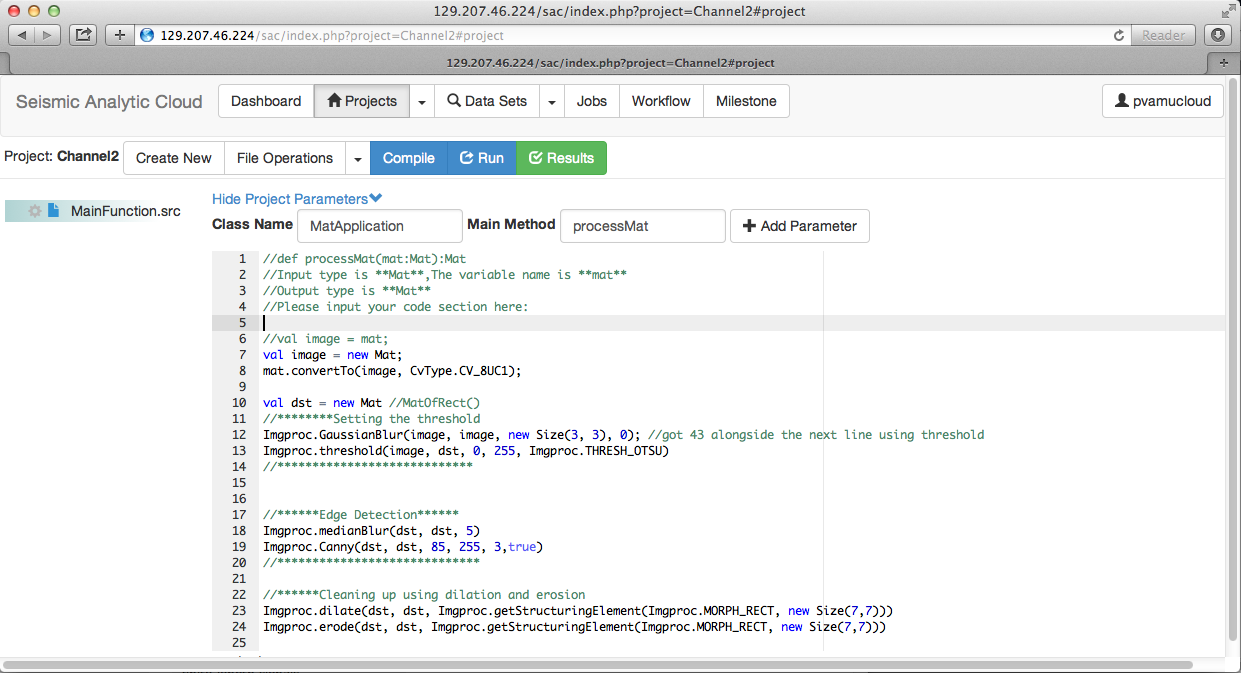
\includegraphics[scale=.35]{figures/Programming.png}
\caption{Programming and Running on Web Interface}
\label{Programming}
\end{figure}
%%%%%%%%%%%%%%%%%%%%%%%%%%%%%%%%%%%%%%%%%%%%%%%%%%%%%%%


%%%%%%%%%%%%%%%%%%%%%%%%%%%%%%%%%%%%%%%%%%%%%%%%%%%%%%%
\begin{figure}[H]
\centering
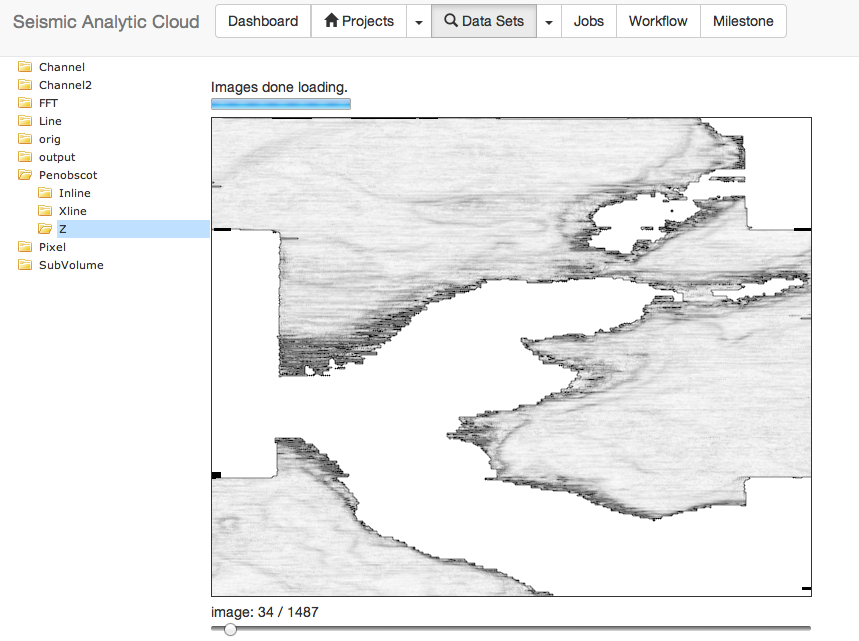
\includegraphics[scale=.45]{figures/DataSet.png}
\caption{Seismic Dataset Preview}
\label{DataSet}
\end{figure}
%%%%%%%%%%%%%%%%%%%%%%%%%%%%%%%%%%%%%%%%%%%%%%%%%%%%%%

%%%%%%%%%%%%%%%%%%%%%%%%%%%%%%%%%%%%%%%%%%%%%%%%%%%%%%%
\begin{figure}[H]
\centering
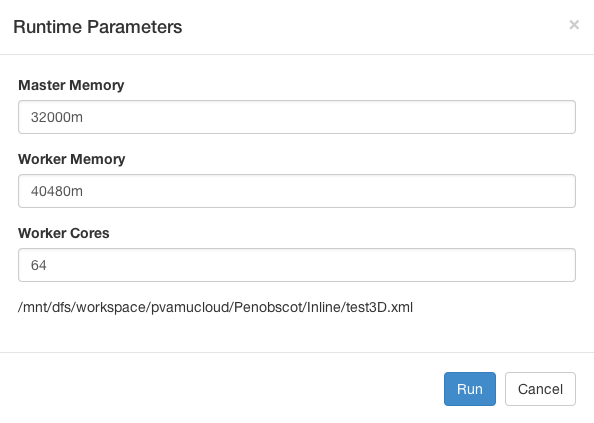
\includegraphics[scale=.60]{figures/Runtime.png}
\caption{Specify runtime parameters}
\label{Runtime}
\end{figure}
%%%%%%%%%%%%%%%%%%%%%%%%%%%%%%%%%%%%%%%%%%%%%%%%%%%%%%

%A table example is going to follow.
\begin{table}[H]
\centering
\caption{Provided UFuncs by ScalaNLP Breeze}
%\begin{tabular}{|p{4cm} |p{8cm} |}
\begin{tabular}{||l|l||}
\hline
Elementwise UFuncs & \shortstack[l]{exp, log, log1p, sqrt, \\sin, cos, tan, asin, acos, atan,\\sinh, cosh, tanh, asinh, acosh, atanh, \\floor, ceil, round, rint, signum, \\abs, isOdd, isEven,sigmoid} \\ 
\hline
Operator UFuncs &  \shortstack[l]{OpAdd: a + b, OpSub: a - b, OpMulMatrix: a * b, \\OpMulScalar: a :* b, OpSolveMatrixBy: a \textbackslash\ b,\\ OpMulInner: a dot b, OpNeg: -a, OpEq: a :== b,\\OpNe: a :!= b, OpLT: a :\textless\ b, OpLTE: a :\textless= b,\\OpGT: a :\textgreater b, OpGTE: a :\textgreater= b, \\OpAnd: a \& b, OpOr: a \textbar\ b, OpNot: !a } \\
\hline
Reduction UFuncs & \shortstack[l]{sum, product, softmax, any, all, \\min, max, argmin, argmax, \\norm, normalize, argsort, argtopk, \\mean, variance, stddev, meanAndVariance }\\
\hline
\end{tabular}
\label{tab:BreezeUFuncs}
\end{table}
%%%%%%%%%%%%%%%%%%%%%%%%%%%%%%%%%%%%%%%%%%%%%%%%%%%%%%

\section{Case Study}
The main characteristics of SAC are productivity, performance, usability and scalability. To prove them, some typical applications in seismic data processing are selected to run on SAC. As for usability and productivity, we will show some codes snippet need to be implemented by end user. As for the performance, executation time of both sequential codes and parallel codes on Spark are compared to get speedup factor, and for scalability, we will configure the running environment with different cores and analyse changing of executation time. To cover more seismic applications, we select four applications as test cases: Calculactor, Transformation, Statistics Functions and Jacobi Stencil codes.

\begin{table}[H]
\caption{Running Time of Sequential Codes with Different Split}
\centering
\begin{tabular}{||c| c c c ||} 
 \hline
 Lines per Split & 12 Lines & 60 Lines & 300 Lines \\ [0.5ex] 
 \hline
 Calculator & 4027 & 4244 & 4613 \\ 
 Hilbert Filter & 7532 & 6257 & 6194 \\
 Histogram & 4858 & 5508 & 5246 \\
 \hline
 \hline
 Subvolume Size & 3x3x3 & 9x9x9 & 17x17x17 \\ [0.5ex] 
 \hline
 FFT & 1395 & 27563 & 596789 \\
 Jacobi & 5972 & 86466 & 463102 \\
 \hline
\end{tabular}
\label{table:CalcSpark}
\end{table}


\subsection{Calculactor}
Calculactor should be the most common used tool in scientific computation. Basic arithmetic operations are easy implemented on normal data, but for big data, the situation is totally different. There are already some commerical and free seismic calculators such as Calculactor in Petrel, Seismic Toolkit listed in \cite{SeismicCalculator} etc. All these seismic calculator are software running on PC, so the performance is bad for handling big seismic data, and most of them even could handle big data. Calculactor designed in SAC is mainly focus on handling big data, in which data is distributed on different nodes and run arithmetic functions in parallel. Most functions in calculator are applied on pixel or sample, and each pixel is a Float type in Scala, so all built-in operator could be used on pixel data. The more convenient way to implement such algorithms are use operators and operations provided by Breeze. For trace or line template in SAC, the data types of input and output are DenseVector and DenseMatrix. ScalaNLP Breeze provide many Universal Functions (UFunc) that can operate on scalars, vectors, matrices, counters with little effort \cite{BreezeUFunc}. All Elementwise UFuncs from scala.math such as exp, log and trigonometric functions etc., and Operator UFuncs such as basic arithmetic, equality and comparison and boolean operations could be applied to DenseVector and DenseMatrix. Table \ref{tab:BreezeUFuncs} shows the functions and operators provided by ScalaNLP Breeze. List \ref{ScalaCode2Line} shows the sample codes of template for processing two Inlines and generate one output Inline.  

\lstset{language=Java,frame=single}
\begin{lstlisting}[float,caption=Sample codes of arighmetic operations on two datasets,label=ScalaCode2Line]

class LineApplication2 extends java.io.Serializable {
    def processLine(line1:DenseMatrix[Double],
                      line2:DenseMatrix[Double])
                      :DenseMatrix[Double] = {
        line1 + sigmoid(ceil(line2)); 
    }
}
\end{lstlisting}

For the performance comparision, the sequential codes are written in Scala and run with single process. Since the volume size of seismic data may so large that could not be fully cached in memory, so the input data set also need to be splited into small parts and be processed one by one and then save back into disk after each part finished. For the parallel codes running on Spark, user only need to write piece of codes in template. The performance of parallel codes may be affected by algorithms, data distributation, number of cores, memory size on each node and speed of communication link etc. 

% put performance index of calculactor here.     

\begin{table}[H]
\caption{Running Time of Calculator on Spark with Different Configurations}
\centering
\begin{tabular}{||c| c c c c ||} 
 \hline
 Split & 72 Cores & 144 Cores & 288 Cores & 576 Cores \\ [0.5ex] 
 \hline
 1 & 915 & 740 & 722 & 724 \\ 
 10 & 212 & 177 & 216 & 442 \\
 30 & 278 & 304 & 387 & 502 \\
 100 & 493 & 453 & 471 & 827 \\
 \hline
\end{tabular}
\label{table:CalcSpark}
\end{table}


\subsection{Fourier \& Hilbert Transformation}
In signal and image processing, Fourier Transform (FT) is the most commonly used algorithm. The signal in time domain was decomposed into a series of frequencies  through FT, and in the frequency domain, many problems sush as filter are easier to perform comparing with in the time domain. Fast Fourier transform (FFT) \cite{FFTWiki} is an algorithm to compute the discrete Fourier transform (DFT) and its inverse by factorizing the DFT matrix into a product of sparse (mostly zero) factors. There are different implementations of FFT, such as FFTW, OpenCV, Kiss FFT, Breeze etc. FFTW\cite{FFTW05} emphasizes performance by adapting to the hardware such as SIMD instructions in order to maximize performance, while Breeze aims to be generic, clean and powerful without sacrificing (much) efficiency. Breeze provide more concise interfaces of 1D/2D Fourier transforms and filtering functions, so we use FFT function in Breeze as test case by applying it both in sequential codes and parallel codes runnning on Spark.     

The Hilbert transform \cite{HilbertWiki} is important in the field of signal processing where it is used to derive the analytic representation of a signal. A great number of geophysical applications consists in close relation of the Hilbert transform to analytic functions of complex variable \cite{HilbertGeoApplication}. Hilbert transform approach now forms the basis by which almost all amplitude, phase and frequency attributes are calculated by today’s seismic interpretation software \cite{HilbertSeismic}. JTK already provided the Hilbert transform filter class, so we use it as test case by apply Hilbert transform filter on each trace of input seismic data set.

Similar to Calculator, we also comparing performance sequential codes on one single node with parallel codes runnning on Spark with different configuration of memory and cores. 

%put performance data of FFT and HTF here.

\begin{table}[H]
\caption{Running Time of Hilbert Transformation Filter on Spark with Different Configurations}
\centering
\begin{tabular}{||c| c c c c ||} 
 \hline
 Split & 72 Cores & 144 Cores & 288 Cores & 576 Cores \\ [0.5ex] 
 \hline
  1 & 5947 & 3312 &	2004 &	1854 \\
  10 & 5230 & 2746 &	1646 &	1628 \\
  30 & 5260 & 2984 &	1839 &	1740 \\
  100 & 5328 & 3357 &	2425 &	2517 \\
 \hline
\end{tabular}
\label{table:HilbertSpark}
\end{table}

\begin{table}[H]
\caption{Running Time of FFT on Spark with Different Configurations}
\centering
\begin{tabular}{||c| c c c c ||} 
 \hline
 Split & 72 Cores & 144 Cores & 288 Cores & 576 Cores \\ [0.5ex] 
 \hline
 3x3x3 & 627 & 355 & 317 & 517 \\ 
 9x9x9 & 506 & 459 & 497 & 700 \\
 17x17x17 & 589 & 532 & 728 & 849 \\
 \hline
 \end{tabular}
 \label{table:FFTSpark}
 \end{table}

\subsection{Statistics functions}
Descriptive statistics is the basis for data analytics, and in seismic data processing, most of statistical functions were already widely used. Spark itself provides some basic reduce functions (also called Actions) such as mean, variance, standard deviation and histogram on RDDs. Besides such basic statistical functions, Breeze also provides a fairly large number of probability distributions used for statistics signal processing. In this test, we use histogram as test case: the sequential codes will iterate whole data samples one by one in one process, and parallel codes will use built-in histogram function in Spark.

%put performance of Histogram here.   

\begin{table}[H]
\caption{Running Time of Histogram on Spark with Different Configurations}
\centering
\begin{tabular}{||c| c c c c ||} 
 \hline
 Split & 72 Cores & 144 Cores & 288 Cores & 576 Cores \\ 
 \hline
  1 & 100 &	64 & 50 & 46 \\
  10 & 216 &	326 & 466 & 639 \\
  30 & 868 &	903 & 819 & 2113 \\
  100 & 1802 & 1766 & 9244 & 8491 \\
 \hline
\end{tabular}
\label{table:HistSpark}
\end{table}

\subsection{Complicate Stencil Operation}

Stencil codes are most common computations used in seismic image processing and reservoir simulation in oil \& gas industry, and most of codes in this domain are written in MPI or OpenMP programming models that running on huge clusters. But MPI codes involve more complexity of programming and could not handle fault tolerance very well, and although OpenMP make it easy to parallelize sequential codes, but with increasing size of volume of seismic data, SMP will encounter problem of caching large data and performance issue for data partition. 
We choose scala as programming language for experiments and develop three applications: Sequential codes, Parallel codes using broadcasting variable and Parallel codes with boundary RDD. For the Sequential codes, we just split the big data file into small splits and each split include several inlines, then using 3 nested loops to compute average value of 26 neighbour samples. After computation, each split will be saved into file to be used as input for next iteration. For the Parallel codes with broadcasting variable, the large input data set are distributed to all active nodes in whole cluster as RDD, then each node could get it own data section and apply map function(computation part) on it. Since boundary data is need for Jacobi kernel and there is no communication interfaces between mappers, the boundary Inlines of each split are collected as a variable and broadcasted to all nodes after one iteration, then each node could fetch new boundary inlines in next iterative computation. After implementation of Parallel codes using broadcasting variable, we found the performance of collecting data is very bad, so we design new Parallel codes using boundary RDDs to exchange boundary data and to avoid collecting data in each iteration. 

The data flow of two parallel methods are shown in Figure \ref{JacobiCode}: Each number denotes one Inline of seismic data. The big seismic data files are stored on HDFS, which will be divided into small splits and send to each node by driver node. Using broadcasting variables shown in top half of diagram, the driver node need collect boundary Inlines from every node, which will take more time on network communication. By changing to boundary RDDs shown in below half diagram, the boundary RDDs are generated from original RDD, but they need repartition and resort for alignment and merge with original RDD to form new RDD.

%%%%%%%%%%%%%%%%%%%%%%%%%%%%%%%%%%%%%%%%%%%%%%%%%%%%%%%
\begin{figure}[H]
\centering
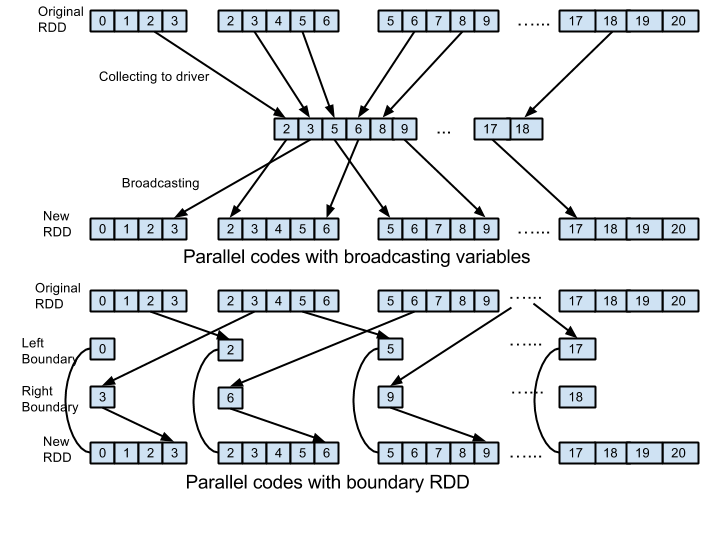
\includegraphics[scale=.6]{figures/JacobiCode.png}
\caption{Data Flow of Jacobi Parallel Codes}
\label{JacobiCode}
\end{figure}
%%%%%%%%%%%%%%%%%%%%%%%%%%%%%%%%%%%%%%%%%%%%%%%%%%%%%%

%put performance of Jacobi here.   

\begin{table}[H]
\caption{Running Time of Jacobi on Spark with Different Configurations}
\centering
\begin{tabular}{||c| c c c c ||} 
 \hline
 Split & 72 Cores & 144 Cores & 288 Cores & 576 Cores \\ [0.5ex] 
 \hline
 3x3x3 & 1384 & 1908 & 1928 & 2239 \\ 
 9x9x9 & 701 & 508 & 409 & 398 \\
 17x17x17 & 196 & 158 & 146 & 150 \\
 \hline
\end{tabular}
\label{table:JacobiSpark}
\end{table}


%%%%%%%%%%%%%%%%%%%%%%%%%%%%%%%%%%%%%%%%%%%%%%%%%%%
%
%  New template code for TAMU Theses and Dissertations starting Fall 2012.  
%  For more info about this template or the 
%  TAMU LaTeX User's Group, see http://www.howdy.me/.
%
%  Author: Wendy Lynn Turner 
%	 Version 1.0 
%  Last updated 8/5/2012
%
%%%%%%%%%%%%%%%%%%%%%%%%%%%%%%%%%%%%%%%%%%%%%%%%%%%

%%%%%%%%%%%%%%%%%%%%%%%%%%%%%%%%%%%%%%%%%%%%%%%%%%%%%%%%%%%%%%%%%%%%%%%
%%%                           SECTION II
%%%%%%%%%%%%%%%%%%%%%%%%%%%%%%%%%%%%%%%%%%%%%%%%%%%%%%%%%%%%%%%%%%%%%%

\chapter{\uppercase {Productivity \& Performance Analysis}}

Text goes here.

\section{Productivity Analysis}
%%%%%%%%%%%%%%%%%%%%%%%%%%%%%%%%%%%%%%%%%%%%%%%%%%%%%%
\begin{figure}[H]
\centering
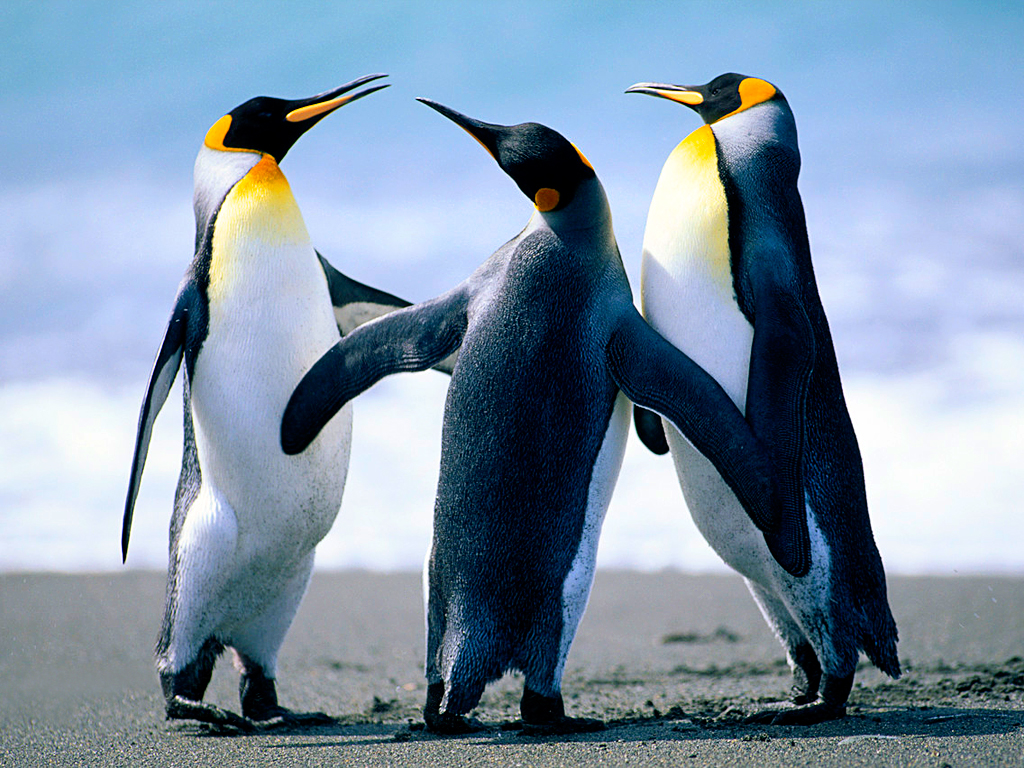
\includegraphics[scale=.50]{figures/Penguins.jpg}
\caption{TAMU figure - This is an example of a long figure title.  Figure titles need to be single-spaced within and double spaced between in the list of figures.}
\label{fig:landscapepenguins}
\end{figure}
%%%%%%%%%%%%%%%%%%%%%%%%%%%%%%%%%%%%%%%%%%%%%%%%%%%%%%
\subsection{Subsection}
\begin{table}[H]
\centering
\caption{This is a table template - This is an example of a long table title.  Table titles need to be single-spaced within and double spaced between in the list of tables.}
\begin{tabular}{|l|c|c|c|c|c|}
\hline
Product & 1 & 2 & 3 & 4 & 5\\
\hline
Price & 124.- & 136.- & 85.- & 156.- & 23.-\\
Guarantee [years] & 1 & 2 & - & 3 & 1\\
Rating & 89\% & 84\% & 51\% & & 45\%\\
\hline
\hline
Recommended & yes & yes & no & no & no\\
\hline
\end{tabular}
\label{tab:template1}
\end{table}


\section{Performance Analysis}




%%%%%%%%%%%%%%%%%%%%%%%%%%%%%%%%%%%%%%%%%%%%%%%%%%%
%
%  New template code for TAMU Theses and Dissertations starting Fall 2012.  
%  For more info about this template or the 
%  TAMU LaTeX User's Group, see http://www.howdy.me/.
%
%  Author: Wendy Lynn Turner 
%	 Version 1.0 
%  Last updated 8/5/2012
%
%%%%%%%%%%%%%%%%%%%%%%%%%%%%%%%%%%%%%%%%%%%%%%%%%%%
%%%%%%%%%%%%%%%%%%%%%%%%%%%%%%%%%%%%%%%%%%%%%%%%%%%%%%%%%%%%%%%%%%%%%%
%%                           SECTION VI
%%%%%%%%%%%%%%%%%%%%%%%%%%%%%%%%%%%%%%%%%%%%%%%%%%%%%%%%%%%%%%%%%%%%%



\chapter{\uppercase{Future Work and Conclusions}}

Text goes here \cite{ApacheHadoop}.

\section{Conclusions}

%%%%%%%%%%%%%%%%%%%%%%%%%%%%%%%%%%%%%%%%%%%%%%%%%%%%%%
\begin{figure}[H]
\centering
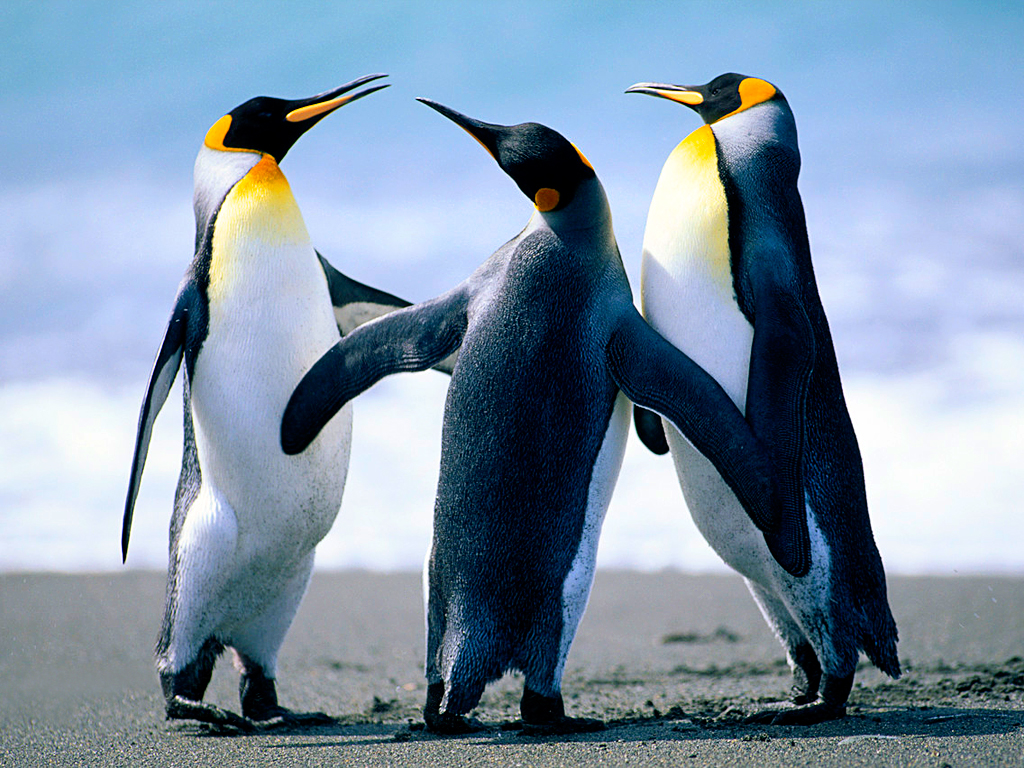
\includegraphics[scale=.50]{figures/Penguins.jpg}
\caption{TAMU figure}
\label{fig:tamu-fig3}
\end{figure}
%%%%%%%%%%%%%%%%%%%%%%%%%%%%%%%%%%%%%%%%%%%%%%%%%%%%%%
\section{Future works}

Text between the figures.  Text between the figures. Text between the figures. Text between the figures.  Text between the figures. Text between the figures. Text between the figures.  Text between the figures. Text between the figures. Text between the figures.  Text between the figures. Text between the figures.
%%%%%%%%%%%%%%%%%%%%%%%%%%%%%%%%%%%%%%%%%%%%%%%%%%%%%%%
%\begin{figure}[H]
%\centering
%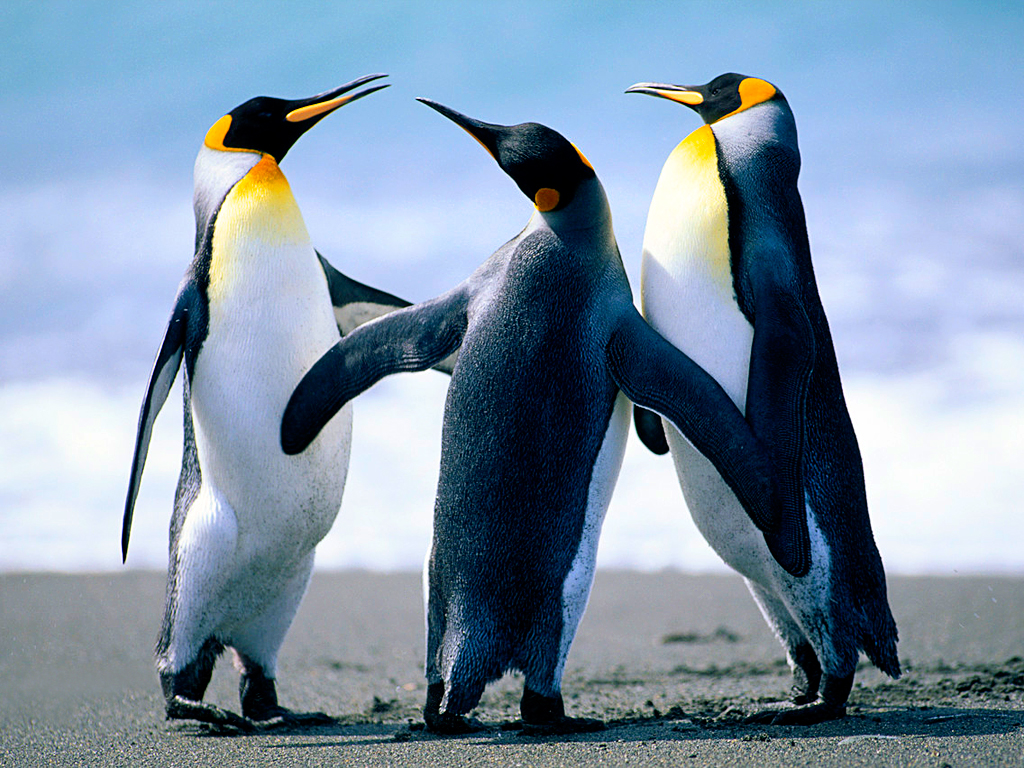
\includegraphics[scale=.50]{figures/Penguins.jpg}
%\caption{Another TAMU figure}
%\label{fig:tamu-fig4}
%\end{figure}
%%%%%%%%%%%%%%%%%%%%%%%%%%%%%%%%%%%%%%%%%%%%%%%%%%%%%%%

\subsection{Subsection}

%%%%%%%%%%%%%%%%%%%%%%%%%%%%%%%%%%%%%%%%%%%%%%%%%%%%%%%
%\begin{figure}[H]
%\centering
%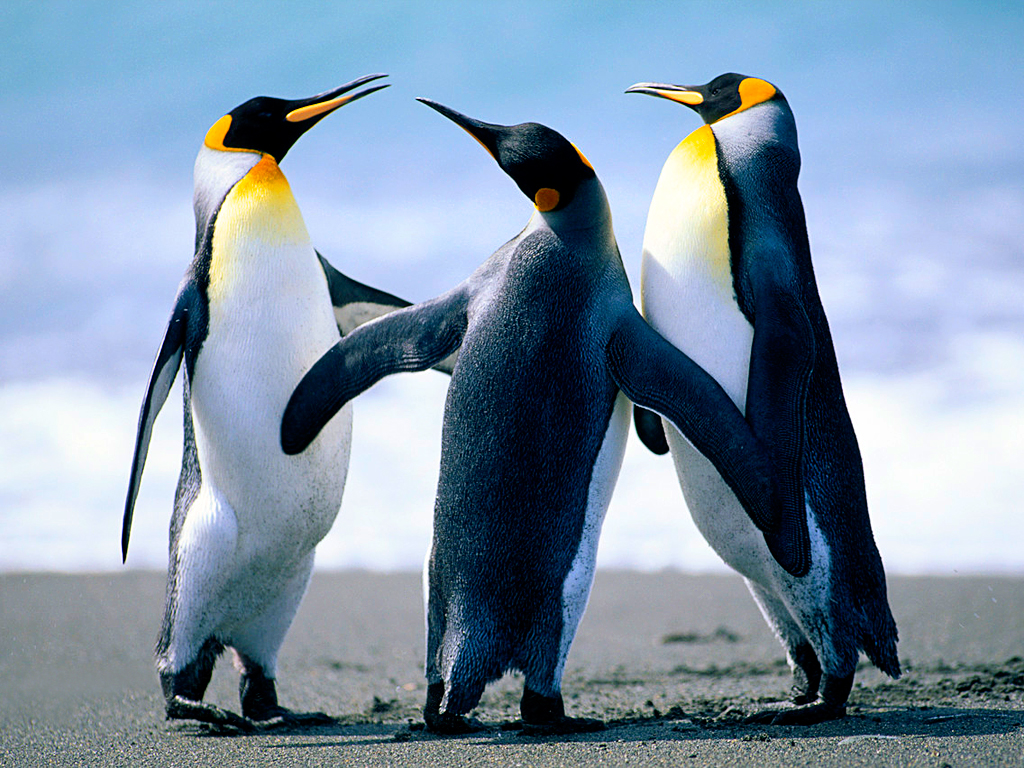
\includegraphics[scale=.50]{figures/Penguins.jpg}
%\caption{Another TAMU figure}
%\label{fig:tamu-fig4-2}
%\end{figure}
%%%%%%%%%%%%%%%%%%%%%%%%%%%%%%%%%%%%%%%%%%%%%%%%%%%%%%%
\subsection{Subsection}

A table example is going to follow.

\begin{table}[H]
\centering
\caption{This is a table template}
\begin{tabular}{|l|c|c|c|c|c|}
\hline
Product & 1 & 2 & 3 & 4 & 5\\
\hline
Price & 124.- & 136.- & 85.- & 156.- & 23.-\\
Guarantee [years] & 1 & 2 & - & 3 & 1\\
Rating & 89\% & 84\% & 51\% & & 45\%\\
\hline
\hline
Recommended & yes & yes & no & no & no\\
\hline
\end{tabular}
\label{tab:template2}
\end{table}
\subsubsection{This is a subsubsection}



%fix spacing in bibliography, if any...
%%%%%%%%%%%%%%%%%%%%%%%%%%%%%%%%%%%%%%%%%%%%%%%%%%%%%%%%%%%%%
\let\oldbibitem\bibitem
\renewcommand{\bibitem}{\setlength{\itemsep}{0pt}\oldbibitem}
%%%%%%%%%%%%%%%%%%%%%%%%%%%%%%%%%%%%%%%%%%%%%%%%%%%%%%%%%%%%%%%
%%%%%%%%%%%%%%%%%%%%%%%%%%%%%%%%%%%%%%%%%%%%%%%%%%%
%
%  New template code for TAMU Theses and Dissertations starting Fall 2012.  
%  For more info about this template or the 
%  TAMU LaTeX User's Group, see http://www.howdy.me/.
%
%  Author: Wendy Lynn Turner 
%	 Version 1.0 
%  Last updated 8/5/2012
%
%%%%%%%%%%%%%%%%%%%%%%%%%%%%%%%%%%%%%%%%%%%%%%%%%%%


%%%%%%%%%%%%%%%%%%%%%%%%%%%%%%%%%%%%%%%%%%%%%%%%%%%%%%%%%%%%%%%%%%%%%%
%%                           REFERENCES 
%%%%%%%%%%%%%%%%%%%%%%%%%%%%%%%%%%%%%%%%%%%%%%%%%%%%%%%%%%%%%%%%%%%%%

\phantomsection
\addcontentsline{toc}{chapter}{REFERENCES}

\renewcommand{\bibname}{{\large\textbf\center REFERENCES}}

\bibliographystyle{plain}
\bibliography{references}

%%%%%%%%%%%%%%%%%%%%%%%%%%%%%%%%%%%%%%%%%%%%%%%%%%%
%
%  New template code for TAMU Theses and Dissertations starting Fall 2012.  
%  For more info about this template or the 
%  TAMU LaTeX User's Group, see http://www.howdy.me/.
%
%  Author: Wendy Lynn Turner 
%	 Version 1.0 
%  Last updated 8/5/2012
%
%%%%%%%%%%%%%%%%%%%%%%%%%%%%%%%%%%%%%%%%%%%%%%%%%%%

\begin{appendices}
\titleformat{\chapter}{\centering\normalsize}{APPENDIX \thechapter}{0em}{\vskip .5\baselineskip\centering}
\renewcommand{\appendixname}{APPENDIX}

%%%%%%%%%%%%%%%%%%%%%%%%%%%%%%%%%%%%%%%%%%%%%%%%%%%
%
%  New template code for TAMU Theses and Dissertations starting Fall 2012.  
%  For more info about this template or the 
%  TAMU LaTeX User's Group, see http://www.howdy.me/.
%
%  Author: Wendy Lynn Turner 
%	 Version 1.0 
%  Last updated 8/5/2012
%
%%%%%%%%%%%%%%%%%%%%%%%%%%%%%%%%%%%%%%%%%%%%%%%%%%%

%%%%%%%%%%%%%%%%%%%%%%%%%%%%%%%%%%%%%%%%%%%%%%%%%%%%%%%%%%%%%%%%%%%%%%
%%                           APPENDIX A 
%%%%%%%%%%%%%%%%%%%%%%%%%%%%%%%%%%%%%%%%%%%%%%%%%%%%%%%%%%%%%%%%%%%%%

\phantomsection

\chapter{\uppercase{First Appendix}}

Text for the Appendix follows.

\begin{figure}[H]
\centering
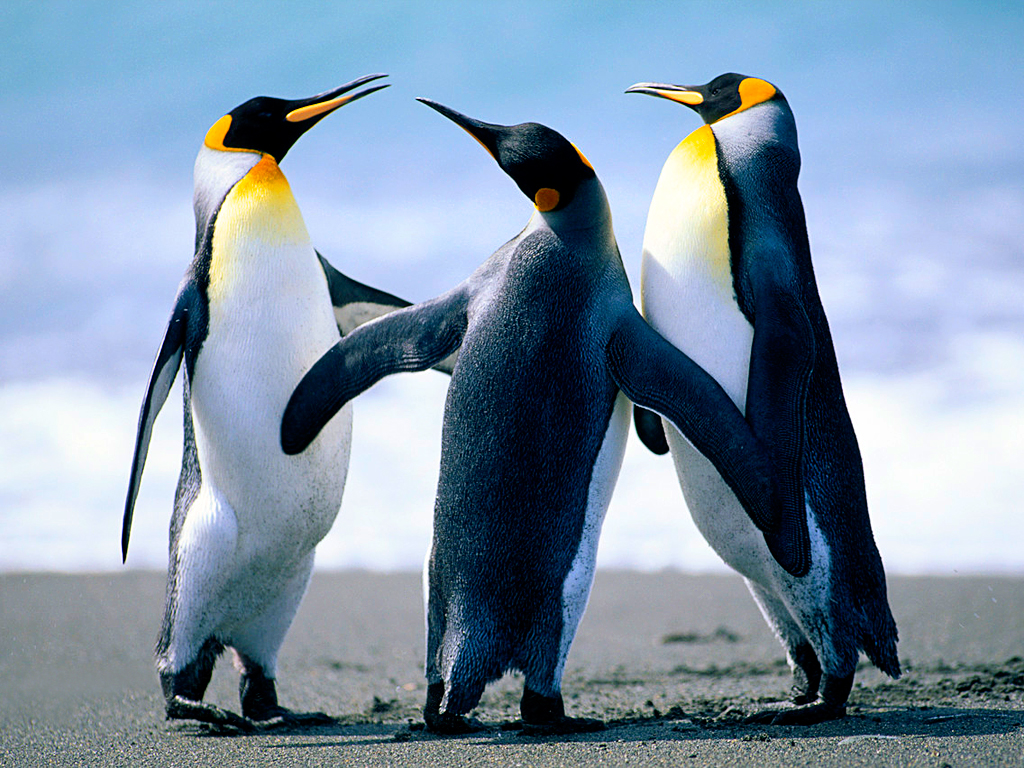
\includegraphics[scale=.50]{figures/Penguins.jpg}
\caption{TAMU figure}
\label{fig:tamu-fig5}
\end{figure}

%%%%%%%%%%%%%%%%%%%%%%%%%%%%%%%%%%%%%%%%%%%%%%%%%%%
%
%  New template code for TAMU Theses and Dissertations starting Fall 2012.  
%  For more info about this template or the 
%  TAMU LaTeX User's Group, see http://www.howdy.me/.
%
%  Author: Wendy Lynn Turner 
%	 Version 1.0 
%  Last updated 8/5/2012
%
%%%%%%%%%%%%%%%%%%%%%%%%%%%%%%%%%%%%%%%%%%%%%%%%%%%

%%%%%%%%%%%%%%%%%%%%%%%%%%%%%%%%%%%%%%%%%%%%%%%%%%%%%%%%%%%%%%%%%%%%%%
%%                           APPENDIX B
%%%%%%%%%%%%%%%%%%%%%%%%%%%%%%%%%%%%%%%%%%%%%%%%%%%%%%%%%%%%%%%%%%%%%

\chapter{\uppercase {Second Appendix with a longer title - much longer in fact}}

Text for the Appendix follows.

\begin{figure}[H]
\centering
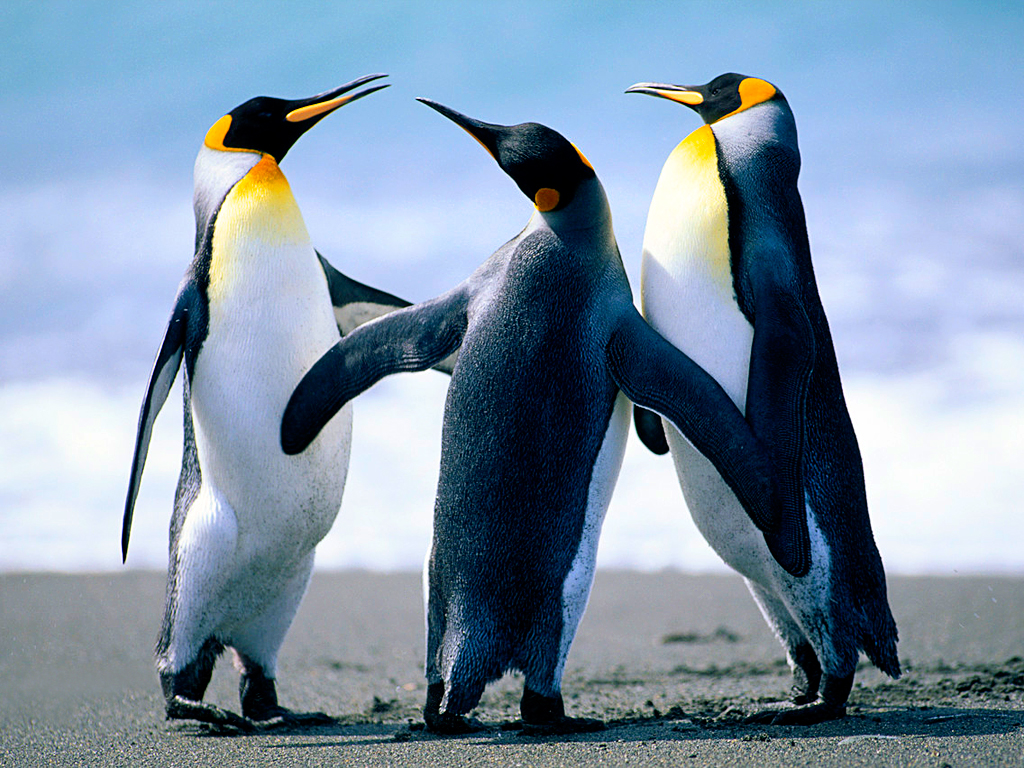
\includegraphics[scale=.50]{figures/Penguins.jpg}
\caption{TAMU figure}
\label{fig:tamu-fig6}
\end{figure}

\section{Appendix Section}


\pagebreak{}

\end{appendices}



\end{document}
